
\documentclass[pdftex,a4paper,12pt]{report}

\usepackage[utf8]{inputenc}  % Accenten gebruiken in tekst (vb. é ipv \'e)
\usepackage{amsfonts}        % AMS math packages: extra wiskundige
\usepackage{amsmath}         %   symbolen (o.a. getallen-
\usepackage{amssymb}         %   verzamelingen N, R, Z, Q, etc.)
\usepackage[dutch]{babel}    % Taalinstellingen: woordsplitsingen,
                             %  commando's voor speciale karakters
                             %  ("dutch" voor NL)
\usepackage{eurosym}         % Euro-symbool €
\usepackage{geometry}
\usepackage{graphicx}        % Invoegen van tekeningen
\usepackage[pdftex,bookmarks=true]{hyperref}
                             % PDF krijgt klikbare links & verwijzingen,
                             %  inhoudstafel
\usepackage{listings}        % Broncode mooi opmaken
\usepackage{multirow}        % Tekst over verschillende cellen in tabellen
\usepackage{rotating}        % Tabellen en figuren roteren
\usepackage{natbib}          % Betere bibliografiestijlen
\usepackage{fancyhdr}        % Pagina-opmaak met hoofd- en voettekst

\usepackage[T1]{fontenc}     % Ivm lettertypes
\usepackage{lmodern}
\usepackage{textcomp}
\usepackage{float}
\usepackage{url}
\usepackage{hyperref}

\usepackage[parfill]{parskip}
\usepackage{fancyhdr}

\usepackage{lipsum}          % Voor vultekst (lorem ipsum)

% \usepackage[parfill]{parskip}
% \usepackage{fancyhdr}

%%---------- Layout ------------------------------------------------------

% hoofdingen, enz.
\pagestyle{fancy}
% enkel hoofdstuktitel in hoofding, geen sectietitel (vermijd overlap)
\renewcommand{\sectionmark}[1]{}

% lijn, wordt gebruikt in titelpagina
\newcommand{\HRule}{\rule{\linewidth}{0.5mm}}

% Leeg blad
\newcommand{\emptypage}{
\newpage
\thispagestyle{empty}
\mbox{}
\newpage
}

% Gebruik een schreefloos lettertype ipv het "oubollig" uitziende
% Computer Modern
\renewcommand{\familydefault}{\sfdefault}

% Commando voor invoegen Java-broncodebestanden (dank aan Niels Corneille)
% Gebruik: \codefragment{source/MijnKlasse.java}{Uitleg bij de code}
\newcommand{\codefragment}[2]{ \lstset{%
  language=java,
  breaklines=true,
  float=th,
  caption={#2},
  basicstyle=\scriptsize,
  frame=single,
  extendedchars=\true
}
\lstinputlisting{#1}}

%%---------- Documenteigenschappen ---------------------------------------
%% Vul dit aan met je eigen info:

% Je eigen naam
\newcommand{\student}{Nathan Baele}

% De naam van je lector, begeleider, promotor
\newcommand{\promotor}{Bert Van Vreckem}

% De naam van je co-promotor
\newcommand{\copromotor}{Selami Top}

% Indien je bachelorproef in opdracht van een bedrijf of organisatie
% geschreven is, geef je hier de naam.
\newcommand{\instelling}{---}

% De titel van het rapport/bachelorproef
\newcommand{\titel}{Beveiliging van een Windows Server 2012 R2 webserver met ASP.NET applicatie}

% Datum van indienen
\newcommand{\datum}{29 mei 2015}

% Faculteit
\newcommand{\faculteit}{Faculteit Bedrijf en Organisatie}

% Soort rapport
\newcommand{\rapporttype}{Scriptie voorgedragen tot het bekomen van de graad van\\Bachelor in de toegepaste informatica}

% Academiejaar
\newcommand{\academiejaar}{2014-2015}

% Examenperiode
%  - 1e semester = 1e examenperiode
%  - 2e semester = 2e examenperiode
%  - tweede zit = 3e examenperiode
\newcommand{\examenperiode}{Tweede examenperiode}

\newcommand*{\captionsource}[2]{%
  \caption[{#1}]{%
    #1%
    \\\hspace{\linewidth}%
    Bron: #2%
  }%
}

%%========================================================================
%% Inhoud document
%%========================================================================

\begin{document} \sloppy

%%---------- Front matter ------------------------------------------------
%% Het voorblad - Hier moet je in principe niets wijzigen.

\begin{titlepage}
  \newgeometry{top=2cm,bottom=1.5cm,left=1.5cm,right=1.5cm}
  \begin{center}

    \begingroup
    \rmfamily
    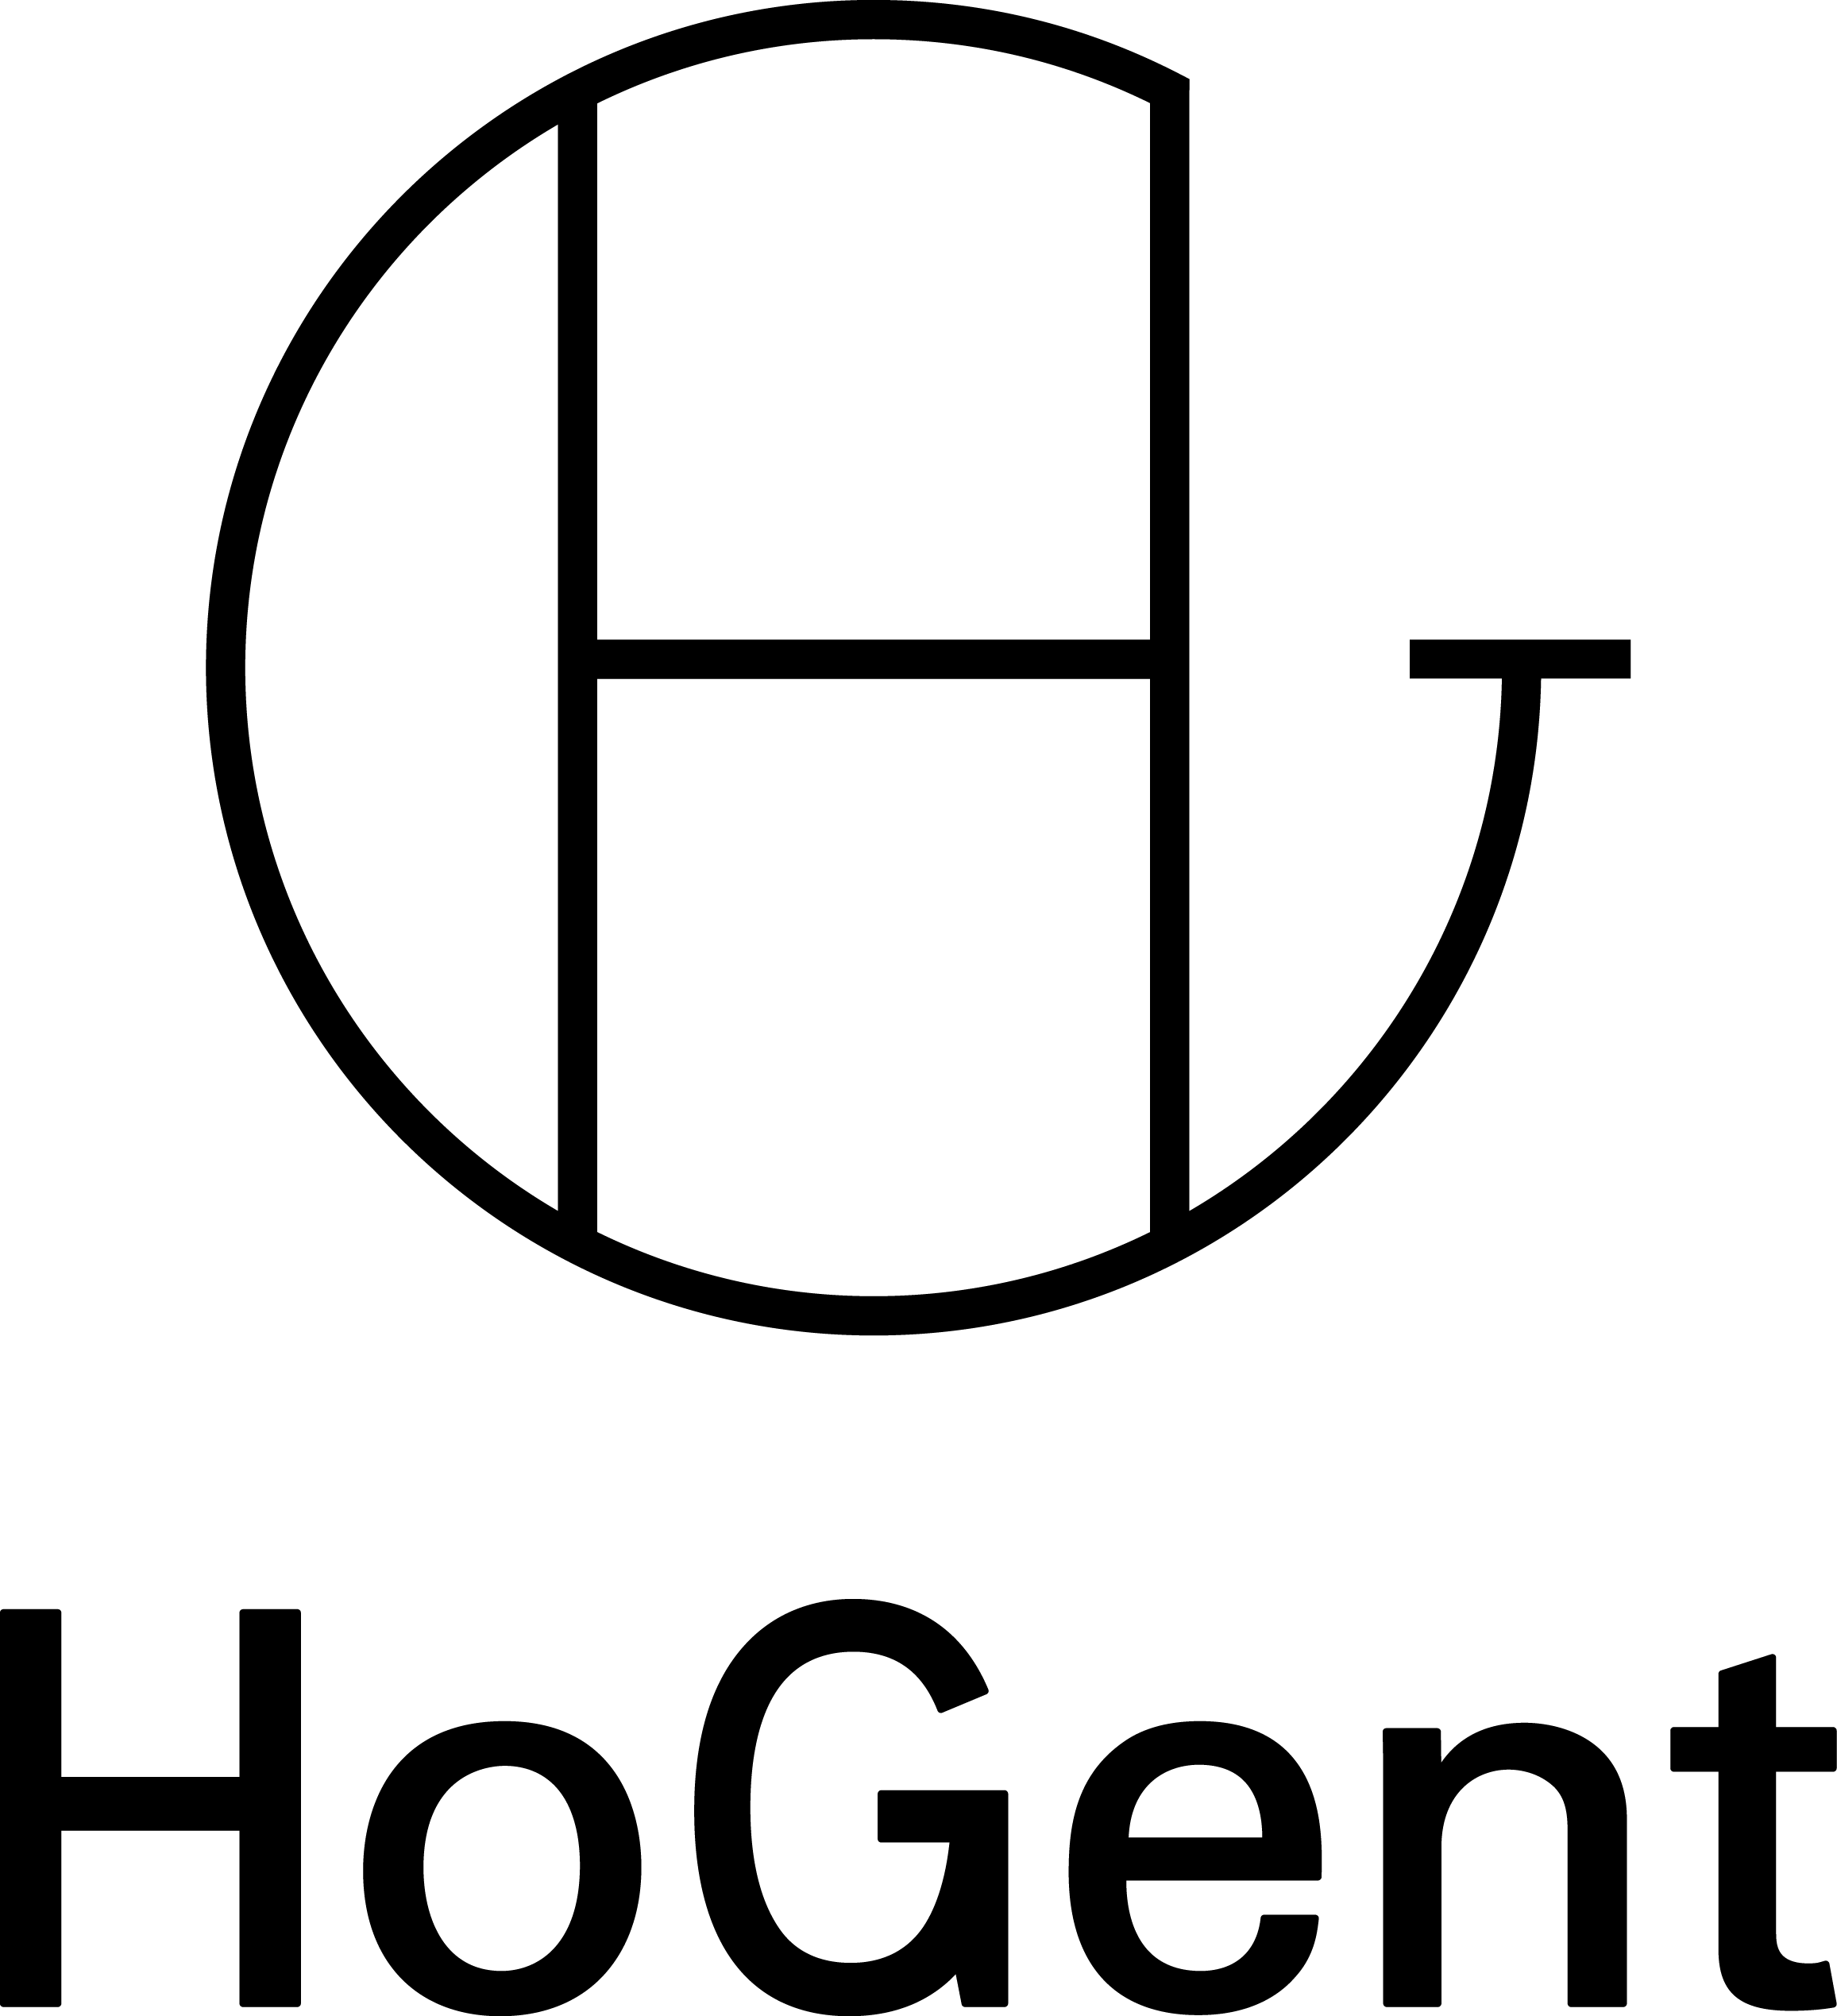
\includegraphics[width=2.5cm]{img/HG-beeldmerk-woordmerk}\\[.5cm]
    \faculteit\\[3cm]
    \titel
    \vfill
    \student\\[3.5cm]
    \rapporttype\\[2cm]
    Promotor:\\
    \promotor\\
    Co-promotor:\\
    \copromotor\\[2.5cm]
    Instelling: \instelling\\[.5cm]
    Academiejaar: \academiejaar\\[.5cm]
    \examenperiode
    \endgroup

  \end{center}
  \restoregeometry
\end{titlepage}

% Schutblad

\emptypage


\begin{titlepage}
  \newgeometry{top=5.35cm,bottom=1.5cm,left=1.5cm,right=1.5cm}
  \begin{center}

    \begingroup
    \rmfamily
    \faculteit\\[3cm]
    \titel
    \vfill
    \student\\[3.5cm]
    \rapporttype\\[2cm]
    Promotor:\\
    \promotor\\
    Co-promotor:\\
    \copromotor\\[2.5cm]
    Instelling: \instelling\\[.5cm]
    Academiejaar: \academiejaar\\[.5cm]
    \examenperiode
    \endgroup

  \end{center}
  \restoregeometry
\end{titlepage}


\begin{abstract}
% TODO: De "abstract" of samenvatting is een kernachtige (max 1 blz. voor een
% thesis) synthese van het document. In ons geval beschrijf je kort de
% probleemstelling en de context, de onderzoeksvragen, de aanpak en de
% resultaten.
Vandaag de dag komt cybercrime meer en meer voor in de bedrijfswereld. Professionele hackers en oplichters proberen binnen te dringen in een netwerk van een bedrijf om gevoelige informatie te gebruiken om zaken te verkrijgen of om het bedrijf op te lichten. Dit probleem groeit even snel als de groei van netwerken in het bedrijfsleven. Daarom is het belangrijk om een zeer goed beveiligd netwerk te hebben tegen bedreigingen van zowel binnen als buiten het bedrijf. \newline 

De doelstelling van dit onderzoek is om een duidelijk overzicht te geven van welke beveilgings best practices er zeker aanwezig moeten zijn op een webserver in een netwerk om beschermd te zijn tegen enkele van de bekendste aanvallen. Na het lezen van deze scriptie zou het mogelijk moeten zijn om zelf een beveilgde webserver op te zetten die voorzien is van deze best practices. \newline

Om dit probleem te onderzoeken heb ik op voorhand enkele onderzoeksvragen vastgesteld. Wat zijn de bekendste soorten van externe en interne bedreigingen en hoe worden deze het efficiëntst opgelost? Hoe word de webserver zo optimaal mogelijk beveiligd? Waar kan een administrator aanvallen terugvinden in de logs?
\end{abstract}

\chapter*{Voorwoord}
\label{ch:voorwoord}
% TODO: Vergeet ook niet te bedankten wie je geholpen/gesteund/... heeft
Deze scriptie zou niet tot stand gekomen zijn zonder de hulp van mijn stagementor en co-promotor Selami Top. Bij het uittesten en onderzoeken van de onderzoeksvragen werd gebruik gemaakt van het netwerk van Hardo bvba, het bedrijf waar Selami Top zaakvoerder van is. Dit zorgde ervoor dat alle conclusies en antwoorden bedrijfsecht zijn en gaf mij een betere kijk op een realistische beveiliging. \newline

Verder wil ik ook mijn promotor Bert Van Vreckem bedanken die mij enorm heeft geholpen met deze bachelorproef tot stand te brengen. Zijn structurele en inhoudelijke tips brachten deze scriptie naar een hoger niveau. Het delen van zijn kennis zorgde er ook voor dat dit onderzoek een betere kwaliteit heeft. \newline

Mijn ouders Johan Baele en Kathleen van Wassenhove zijn ook een grote hulp geweest. Deze hebben mij enorm gesteund tijdens het onderzoeken van dit onderwerp en hebben mij geholpen met het nalezen van de eindtekst en het verbeteren van enkele taal -en layoutfouten. \newline

Tot slot wil ik alle auteurs bedanken van de boeken, websites, handleidingen, videolessen, ... die ik heb gelezen. Dankzij hun bijdrage is de kwaliteit van deze scriptie en mijn kennis enorm verbeterd. 


\tableofcontents

% Als je een lijst van afkortingen of termen wil toevoegen, dan hoort die
% hier thuis. Gebruik bijvoorbeeld de ``glossaries'' package.

%%---------- Kern --------------------------------------------------------

\chapter{Inleiding}
\label{ch:inleiding}
"`The bad guys are winning"'. Met deze woorden in een artikel van \cite{Wiener-Bronner2014} is het duidelijk dat vandaag de dag cybercrime meer en meer voorkomt. Professionele hackers en oplichters proberen binnen te dringen in een netwerk/server van een bedrijf om gevoelige informatie te verkijgen en te gebruiken om het bedrijf op te lichten. Daarom is het belangrijk om een zeer goed beveiligd netwerk te hebben tegen bedreigingen van zowel binnen als buiten het bedrijf en dat is ook één van de doelstellingen in dit onderzoek. \newline

In deze scriptie zal een fictief netwerk opgezet worden dat een domeincontroller en een webserver zal bevatten. Deze beide virtuele machines zullen geconfigureerd worden volgens de algemene best practices om zo de beveiliging van deze servers te verbeteren. Er zijn natuurlijk honderden verschillende soorten aanvallen en mogelijkheden tot cybercrime of tot het binnendringen van een netwerk. Enkele van de meest voorkomende aanvallen zijn SQL-injectie, exploits \citep{Siddharth2006}, DDoS, port scans en social engineering \citep{Gibson2011}, maar er zijn nog immens veel soorten.

Er moet dus ergens een keuze gemaakt worden welke aanvallen er in dit onderzoek zullen besproken worden. Dit zal gebeuren a.d.h.v. een risico-analyse van de webserver om te kijken welke aanvallen het meeste kans hebben om uitgevoerd te worden en dus van belang zijn. De aanvallen die de grootste kans hebben of die het meeste schade kunnen toebrengen aan de webserver zullen dan later in dit onderzoek één voor één besproken worden. \newline 

Deze aanvallen zullen dan ook uitgevoerd worden met een Kali Linux-aanvallersmachine tegen de webserver om te kijken of de eerder geïmplementeerde best practices voldoende zijn om de server te beveiligen, of dat er extra maatregelen moeten getroffen worden. Dit heeft niet alleen als doel om de best practices aan te vullen en te verbeteren, maar ook om de typische aanpak van beveilingsproblemen waar er enkel wordt gehandeld nadat er iets is gebeurd te vermijden. Het probleem hierbij is dat er niet preventief wordt nagedacht en dat er al een aanval is uitgevoerd voordat er naar een oplossing wordt gezocht. Dit kan resulteren in schade of diefstal binnen het netwerk en zo is het dus belangrijk dat het ad-hoc controleren op fouten niet de meest gebruikte beveiligingsmanier is. \newline

Tot slot wordt er gekeken naar hoe de administrator deze aanvallen kan terugvinden in de logs als ze zijn uitgevoerd of nog bezig zijn. Er kan altijd een aanval door de bevieliging geraken en dan is het belangrijk om snel en goed te reageren. Hoe sneller dat een aanval gesignaleerd wordt, hoe sneller er ook een oplossing kan gevonden worden. Dit is cruciaal om toekomstige aanvallen af te weren want hoe langer een zwakte na een aanval onopgelost blijft, hoe meer risico er is dat er meerdere aanvallen zullen plaatsvinden. Dus het maken van geautomatiseerde logs en scans kan ervoor zorgen dat problemen bijna direct worden opgemerkt.


\section{Probleemstelling en Onderzoeksvragen}
\label{sec:onderzoeksvragen}

% TODO: Wees zo concreet mogelijk bij het formuleren van je
% onderzoeksvra(a)g(en). Een onderzoeksvraag is trouwens iets waar nog
% niemand op dit moment een antwoord heeft (voor zover je kan nagaan).
\subsection{Zijn de best practices voldoende als beveiliging tegen een externe of interne aanval?}

Allereerst wordt de webserver geconfigureerd volgende de best practices van \cite{Cott2012}, \cite{Microsoft2013}, \cite{Poley2013}, \cite{Posey2011} en \cite{Vialle2012}. Daarna wordt er een risico-analyse uitgevoerd en wordt er gekeken naar welke aanvallen relevant zijn en verder zullen onderzocht worden. Deze selectie van aanvallen zullen uitgevoerd worden om te kijken of de geïmplementeerde best practices voldoende zijn om de server te beveiligen of dat er aanvullingen moeten gedaan worden. 

\subsection{Wat is de beste manier om als administrator sporen terug te vinden van een aanval?}

Het spreekt voor zich dat, wanneer er zich een aanval voordoet of heeft voorgedaan, dat een netwerkbeheerder dit direct of toch zo snel mogelijk wilt te weten komen. Als er een aanval gaande is dan is het belangrijk dat de beheerder dit snel weet en dat deze snel de oorzaak vindt en weet wat er precies aan het gebeuren is. Hetzelfde geldt voor wanneer er een aanval heeft plaatsgevonden in de geschiedenis. Het is de taak van de administrator om ervoor te zorgen dat aanvallen makkelijk terug te vinden zijn ofwel manueel ofwel automatisch zodat deze tijdig kunnen onderbroken worden of niet meer zullen voorvallen.

\chapter{Methodologie}
\label{ch:methodologie}

% TODO: Hoe ben je te werk gegaan? Verdeel je onderzoek in grote fasen, en
% licht in elke fase toe welke stappen je gevolgd hebt. Verantwoord waarom je
% op deze manier te werk gegaan bent. Je moet kunnen aantonen dat je de best
% mogelijke manier toegepast hebt om een antwoord te vinden op de
% onderzoeksvraag.

Dit onderzoek bestaat uit de volgende methodiek:
\begin{enumerate}
	\item Een dergelijke basiskennis is vereist dus het verrichten van onderzoek en lezen van lectuur is een essentiële eerste stap.
	\item Opzetten van een goede testomgeving met één Windows Server 2012 R2 domeincontroller, één Windows Server 2012 R2 webserver met ASP.net-applicatie draaiende als slachtoffer en één Kali Linux-machine als aanvaller. De Webserver zal geconfigureerd worden volgens de best practices.
	\item Een risicoanalyse uitvoeren en kijken wat de belangrijkste bedreigingen zijn voor dit type systemen.
	\item Met behulp van penetration testing tools beveiligingsproblemen zoeken en uitbuiten. Hier wordt er vanuit gegaan dat er geen fysieke toegang is tot de server dus een boot-cd insteken, rebooten en het administrator wachtwoord wijzigen zal niet lukken. Er wordt een lijst gemaakt met welke aanvallen er gaan gedaan worden en welke succesvol worden uitgevoerd en welke falen. Indien een aanval succesvol wordt uitgevoerd, dan zullen de best practices moeten aangevuld worden.
	\item Het uitvoeren van een post-mortem om sporen van inbraak bloot te leggen en kijken waar het probleem zich bevindt.
\end{enumerate}

\begin{figure}[H]
\begin{center}
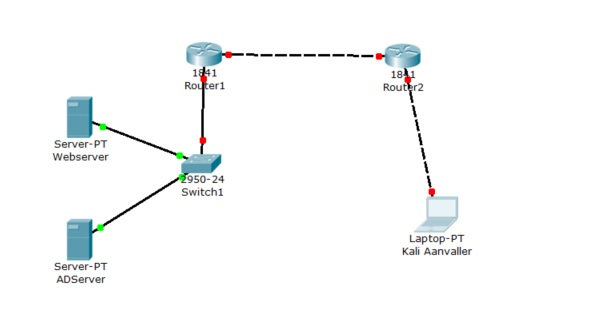
\includegraphics{img/Situatie}
\end{center}
\caption{Proefopstelling}
\label{img:situatie}
\end{figure}

In figuur~\ref{img:situatie} is te zien welke machines allemaal nodig zijn om dit onderzoek tot een goed einde te brengen. Ten eerste is er een Active Directory-server nodig die ook domeincontroller is in het domein en deze server is ook nog DNS-server ook. Dan is er de webserver die lid is van hetzelfde domein als de ADServer natuurlijk. Deze zijn aangesloten aan een switch en een router. Ten slotte is er ook nog een aanvallersmachine om te proberen de server te hacken. Deze is ook aangesloten aan een router op een andere locatie. Tot slot wordt er gebruik gemaakt van VMWare Workstation om al deze virtuele machines te maken met elkaar te verbinden.

%% TODO: de structuur en titel van deze hoofdstukken hangen af van je
% eigen onderzoek. Elke fase in je onderzoek kan een eigen hoofdstuk krijgen. Kies telkens een gepaste titel. ``Corpus'' is *GEEN* gepaste titel
\chapter{Opzetten servers met best practises beveiliging}
%Hier ga ik schrijven over wat de best practises zijn om een webserver te beveiligen en ga ik zeggen hoe je deze moet configureren/implementeren
\section{Installatie + configuratie ADServer}
De Windows Server 2012 R2-virtuele machine genaamd "`ADServer"' is de eerste die moet worden opgezet. In VMWare Workstation wordt er 60GB geheugen gealloceerd voor deze virtuele machine samen met één netwerkadapter en 2GB aan RAM-geheugen. Nadat Windows Server 2012 R2 is geïnstalleerd op deze virtuele machine, krijgt deze de naam "`ADServer"' en wordt deze heropgestart. Daarna kan er begonnen worden met het installeren van de nodige rollen. De eerste rol die wordt geïnstalleerd is de rol textit{Active Directory Domain Services}. Daarna wordt de ADServer opgewaardeerd naar domeincontroller in het fictieve domein "`Baele.be"'. Op de server is één netwerkadapters aanwezig en deze wordt handmatig ingesteld. De server krijgt als IP-adres 192.168.1.2 mee, als subnetmask 255.255.255.0, als default gateway 192.168.1.2 en als DNS-server 127.0.0.1. \newline

Het volgende dat moet gebeuren is het installeren en configureren van de DNS-rol. Dit is vrij simpel en neemt niet veel tijd in beslag. In het scherm "`DNS-beheer"' wordt er in het tabblad "`Zones voor reverse lookup"' een zone aangemaakt met de naam "`1.168.192.in-addr.arpa"' en daarna wordt er een PTR-record aangemaakt die verwijst naar de net geconfigureerde LANadapter met het juiste IP-adres. Hierna wordt de DHCP-rol geïnstalleerd en wordt er een nieuwe scope aangemaakt met de naam "`TestScope"'. Het eerste IP-adres in het bereik is 192.168.1.1 en het laatste 192.168.1.254. De adressen van 192.168.1.1 tot 192.168.1.20 worden uitgesloten voor distributie. De WebServer wordt de router dus het IP-adres dat hier wordt meegegeven is 192.168.1.3. Dit is het IP-adres die later aan de router/WebServer wordt gegeven. \newline

\section{Installatie + configuratie WebServer}
De installatie start op dezelfde manier als de voorgaande machine, maar in dit geval wordt de machine \textit{WebServer} genoemd en zijn er twee netwerkadapters aanwezig, één die is verbonden met het internet (Internetadapter) en een andere die is verbonden met het LAN (LANadapter). De internetadapter staat geconfigureerd als NAT en de IP -en DNS-informatie worden alletwee automatisch aangewezen. Bij de LANadapter zijn de instellingen anders, hier staat deze configureerd als \textit{Custom: specific virtual network} en wordt er gekozen om het virtuele network de naam \textit{VMnet0} mee te geven. Hierdoor moeten de IP -en DNS-instellingen handmatig geconfigureerd worden. De server krijgt al IP-adres 192.168.1.2 mee, als subnetmask 255.255.255.0, als default gateway 192.168.1.2 en als DNS-server 127.0.0.1. \newline 

Deze server wordt ook lid gemaakt van het domein \textit{Baele.be}. Verder wordt er ook de rol \textit{Externe Toegang} toegevoegd. Deze stellen we zo in dat de netwerkadapter waar het internet van komt wordt gebruikt voor andere hosts die verbonden zijn met het netwerk en die op het internet moeten. De WebServer wordt dus zo een router. \newline

Op deze server is het belangrijk dat de rol \textit{Internet Information Service 8} (IIS8) is geïnstalleerd. Deze is al automatisch geïnstalleerd bij het installeren van de rol \textit{Externe Toegang}. Verder is de installatie van databanksoftware ook nodig. In dit geval wordt er gebruik gemaakt van Microsoft SQL Management Studio 2014. Bij de installatie is het aangeraden om \textit{Use Microsoft Update to check for updates} aan te vinken. Na de installatie wordt er een testdatabase aangemaakt met de naam \textit{TestDatabase} en in deze database wordt er een tabel aangemaakt met de naam \textit{People} met de rijen \textit{PeopleID, Fname, Lname} en steek twee willekeurige waarden in deze tabel. Tot slot wordt er nog een nieuwe stored procedure aangemaakt met de volgende inhoud:
\begin{verbatim}
Create Procedure Test_GetPeople
AS
Select * from People;
\end{verbatim}

De volgende stap is om een basis ASP.net-applicatie te maken en dit wordt gedaan met de hulp van \cite{Nuckolls2011}. Met behulp van deze persoon zijn tutorial, de link is te vinden in de bibliografie, is er direct een ASP.net-applicatie met een achterliggende database toegevoegd. \newline

\section{Installatie + configuratie aanvallersmachine}
De derde en laatste virtuele machine die nodig is in dit onderzoek is de Kali Linux-aanvallersmachine. Deze is vrij makkelijk te installeren en heeft ook niet zo hoge systeemvereisten. Voor deze machine is er maar 20Gb aan gealloceerd geheugen nodig samen met 1 netwerkadapter die op \textit{VMnet0} staat en 512MB aan RAM-geheugen. Bij het starten van de installatie moet er gekozen worden voor \textit{graphical install}. De meeste stappen zijn voor de hand liggend, maar bij partition disks wordt er \textit{guided-use entire disk} het best geselecteerd. De naam van de machine wordt ingesteld op \textit{KaliAanvaller}. Op het moment dat er wordt gevraagd van welk netwerk deze computer deel uit maakt, wordt er \textit{baele.be} gekozen. Voor de rest zijn de overige stappen niet zo belangrijk en is de installatie zo afgerond.

\section{Besturingssysteem best practices WebServer}
Nu dat de webserver is geïnstalleerd, kan er begonnen worden aan het toepassen van de best practices. Het is zeer belangrijk dat dit eerst wordt gedaan voordat de server wordt opgenomen in het netwerk. In dit deel worden alle best practices van het besturingssysteem besproken van een sterk wachtwoordbeleid tot het regelmatig updaten van de server.
\subsection{Wachtwoordbeleid}
\subsubsection{Wachtwoord geschiedenis afdwingen}
Dit is een policy die ervoor zorgt dat gebruikers, als ze van wachtwoord moeten veranderen, ze niet kunnen wisselen tussen altijd dezelfde wachtwoorden. Er kunnen in totaal tot wel 24 wachtwoorden opgeslaan worden in de wachtwoordgeschiedenis dus zo is de kans klein dat gebruikers blijven wisselen tussen dezelfde wachtwoorden. Als een gebruiker slim is kan hij zijn wachtwoord gewoon 24 keer na elkaar wijzigen om dan terug zijn oude antwoord te gebruiken. Dit kan ook voorkomen worden door een \textit{Minimum Password Age Policy} in te stellen zodat een wachtwoord bijvoorbeeld maar om de 2 dagen kan veranderd worden. \citep{Stanek2009} \newline

Dit kan geïmplementeerd worden door naar het \textit{Lokaal beveiligingsbeleid} te gaan en daar te klikken op het \textit{Wachtwoordbeleid}. Er is te zien dat de \textit{Minimale wachtwoordduur} default staat ingesteld als 1 dag en de wachtwoordgeschiedenis op 24 wachtwoorden dus dit mag zo gelaten worden als best practice.

\subsubsection{Wachtwoord regelmatig wijzigen}
Een andere best practice is om het wachtwoord regelmatig eens te veranderen. Dit kan mondeling gebeuren, maar het meest efficiënte is om dit ook te doen a.d.h.v. een policy. Er kan terug gegaan worden naar de voorgaande locatie en daar kan er gekozen worden voor \textit{Maximale wachtwoordduur}. Deze staat default op 42 dagen dit is een goede waarde voor netwerken waar beveiliging zeer belangrijk is want daar wordt er meestal gekozen voor een waarde tussen de 30-90 dagen. Bij netwerken waar de beveiliging niet zo belangrijk is kan dit eerder 120-180 dagen zijn. \citep{Stanek2009}

\subsubsection{Minimale wachtwoordlengte}
Deze policy, die ook te vinden is op dezelfde plek als de vorige policies, zorgt ervoor dat een gebruiker zijn wachtwoord minimaal een bepaalde lengte moet hebben. Dit heeft als bedoeling om het brute force kraken van wachtwoorden moeilijker tot onmogelijk te maken. Default staat deze policiy op 7 dagen maar \cite{Stanek2009} raadt aan om deze policy in te stellen op een lengte van minstens 14 tekens. Dit heeft als reden dat een wachtwoord van 7-8 tekens vandaag de dag op een korte tijd wordt gekraakt door het toepassen van brute force wachtwoord kraken met mdoerne hardware.

\subsubsection{Complexiteit van het wachtwoord}
Het spreekt voor zich dat een wachtwoord zoals \textit{123456} niet acceptabel is. Daarom is het belangrijk dat er een policy is die de complexiteit van een wachtwoord verzekerd. Dit kan alweer gevonden worden op voorgaande locatie waar de policy \textit{Wachtwoorden moeten voldoen aan complexiteitsvereisten} kan worden ingeschakeld. Dit zorgt ervoor dat de wachtwoorden minstens 6 tekens moeten hebben, er kunngen geen gebruikersnamen of gewone namen in voorkomen en wachtwoorden moeten minstens 3 van de 4 verschillende soorten karaktertypes bevatten (normale letters, hoofdletters, nummers en symbolen). \citep{Stanek2009}

\subsection{Accountbeheer}
\subsubsection{Uitschakelen van Administrator-account}
Eén van de eerste zaken dat moet gebeuren is het uitschakelen van de inlognaam \textit{Administrator}. Dit heeft als reden dat elke persoon weet dat het default account deze naam heeft en zo is het voor hackers gemakkelijker om binnen te breken als deze al de naam van een account met administrator rechten bezitten. Dit account kan uitgeschakeld worden door op de ADServer naar de \textit{Active Directory - gebruikers en computers} te gaan en daar bij \textit{Users} en daar te rechterklikken op het account \textit{Administrator} en deze dan uit te schakelen.

\subsubsection{Aanmaken eigen administrator-account}
Nadat in de vorige stap het default administrator-account is uitgeschakeld, moet er natuurlijk weer een nieuw account komen zodat er toch nog administrator-taken kunnen uitgevoerd worden. Dit kan gedaan worden door op dezelfde locatie als de voorgaande stap een nieuwe gebruiker toe te voegen, in dit geval met de naam \textit{BaeleAdministrator}, en deze lid te maken van de groepen \textit{Administrators, Domeinadministrators en domeincontrollers}. Nu is het best om even uit te loggen en terug in te loggen met het nieuwe account.

\subsection{Updates}
Nog een belangrijke onderdeel van een server met best practice beveiliging, is het regelmatig downloaden en installeren van updates. Bij het vinden van een nieuw zwak punt of exploit in software, wordt dit al binnen enkele uren op het internet geplaatst en wordt er dus ook gewerkt aan een oplossing. Als de server en applicaties continue worden geupdate, dan is de kans veel kleiner dat er een exploit zal uitgebuit worden. \citep{Cott2012}. Automatische updates worden echter zo goed als nooit gedaan. De voorgestelde updates worden best door de administrator gedownload en uitgetest in een virtuele testomgeving zodat er zekerheid is dat deze update geen problemen met zich meebrengt. Nadat deze test is geslaagd, kan de update op de webserver geïnstalleerd worden.

\subsection{Backup}
Het maken van geautomatiseerde backups is essentieel voor een server binnen een netwerk. Een fout, probleem of aanval kan elke moment van de dag gebeuren en als dit gebeurt moet het mogelijk zijn om het systeem terug te zetten van een eerder gemaakte backup. In de Windows Server Backup-wizard kan dit worden ingesteld voor elke harde schijf. In dit geval wordt er enkel elke nacht om 03:00u een back-up genomen van de C-schijf, maar dit varieert van bedrijf tot bedrijf en hangt af van hoeveel geheugen er beschikbaar is voor back-ups en welke dataschijven het belangrijkste zijn. 

\subsection{Firewall}
De firewall is enorm belangrijk en heeft vooraf al een configuratie meegekregen. Er is echter één aanpassing van de configuratie die in de praktijk veel wordt toegepast en die ook door \cite{Nabors2013} wordt genoemd als een best practise-instelling voor een Firewall-configuratie. Dit betreft het blokkeren van alle uitgaande verbindingen die niet overeenkomen met één van de gedefinieerde regels. \newline 

Dit wordt gedaan door naar de eigenschappen te gaan en daar in alledrie de profielen de uitgaande verbindingen op "`blokkeren"' te zetten. Standaard staat dit geconfigureerd als "`toestaan"'. Hierna kunnen er eigen inkomende en uitgaande regels geconfigureerd worden naargelang de applicaties die op de server komen te staan en welke poorten open of dicht moeten zijn. Bij uitgaande verbindingen is het belangrijk dat de TCP-poorten 80 (hhtp) en 443 (https) worden toegevoegd aan de uitzonderingen. Nadat deze poorten zijn toegevoegd dan ziet de verzameling van toegestane uitgaande verbinden eruit als in figuur~\ref{img:FirewallUitgaand} te zien is.

\begin{figure}[H]
\begin{center}
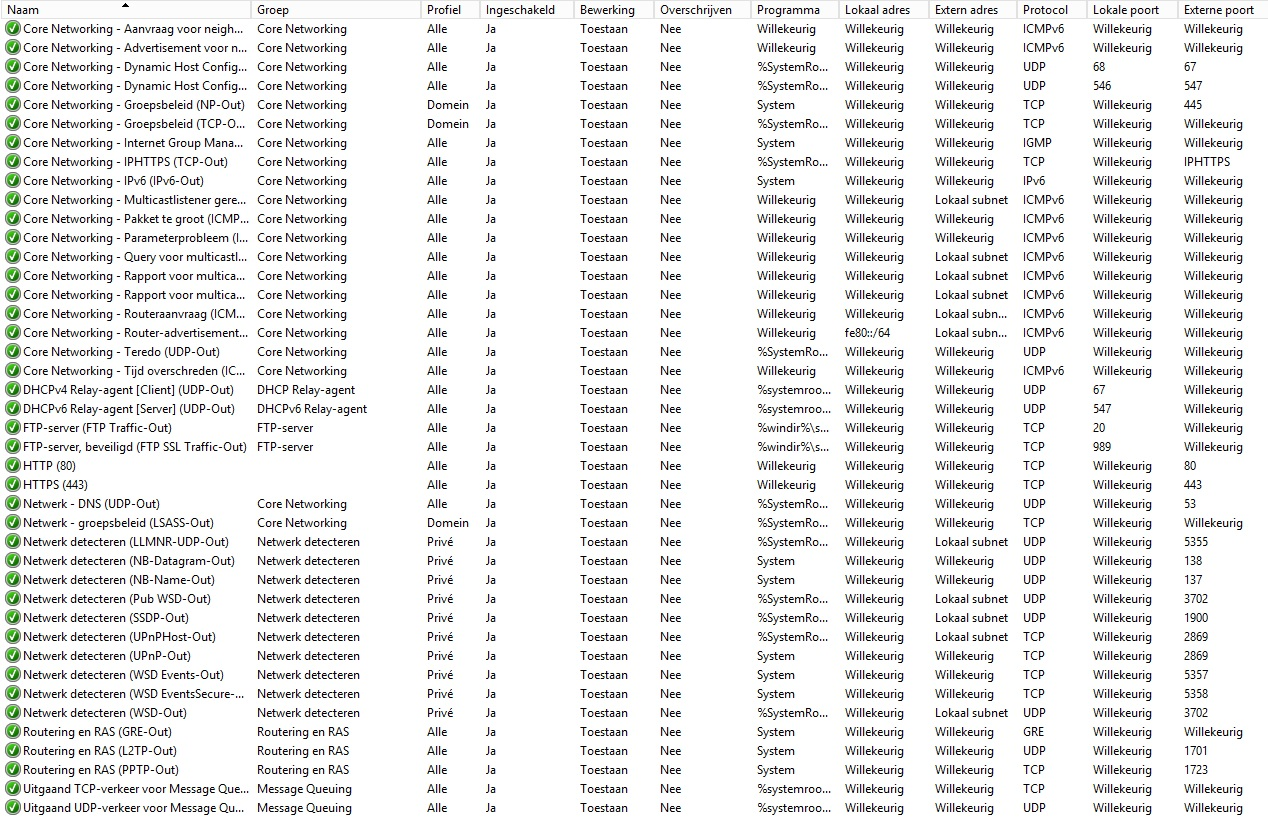
\includegraphics[scale=0.45]{img/FirewallUitgaand}
\end{center}
\caption{Alle toegestane uitgaande verbindingen}
\label{img:FirewallUitgaand}
\end{figure}

\subsection{Anti-virus}
\subsubsection{Goede anti-virus installeren}
Een degelijke anti-virus is enorm belangrijk om een server, computer of ander online apparaat te beschermen. Bij het gebruiken van een desktop of laptop voor persoonlijk gebruik, is een gratis versie van een bepaalde anti-virus-software voldoen. Voor in een bedrijfsomgeving is het beter dat er een betaalde versie wordt genomen aangezien deze veel meer functies en opties hebben. Microsoft heeft een gratis beveiligingssoftwarepakket genaamd \textit{Microsoft Security Essentials}, maar deze heeft geen versie voor op de Windows Server 2012-besturingssystemen te worden geïnstalleerd. Dit wil niet zeggen dat de installatie van deze software niet lukt natuurlijk op een Windows server.

Allereerst moet er gegaan worden naar de website van Microsoft Security Essentials om daar de recentste versie te downloaden en dit voor een Windows 7 64-bit machine. Als deze installer is gedownload dan moet er gegaan worden naar de eigenschappen om daar de compatibiliteit te veranderen naar Windows 7. Hierna moet er een opdrachtprompt gestart worden en moet er genavigeerd worden naar de map waar de installer is in geplaatst. Daar wordt er met het volgende lijntje \begin{verbatim} mseinstall /disableoslimit \end{verbatim} de installer succesvol gestart. Bij de installatie hoeft er enkel op \textit{volgende} gedrukt te worden en de software wordt succesvol geïnstalleerd. Hierna kan er een eerste scan worden gestart die de hele server onderzoekt op virussen en spyware nadat deze zichzelf heeft bijgewerkt met de nieuwste updates. \citep{Herring2014}

\begin{figure}[H]
\begin{center}
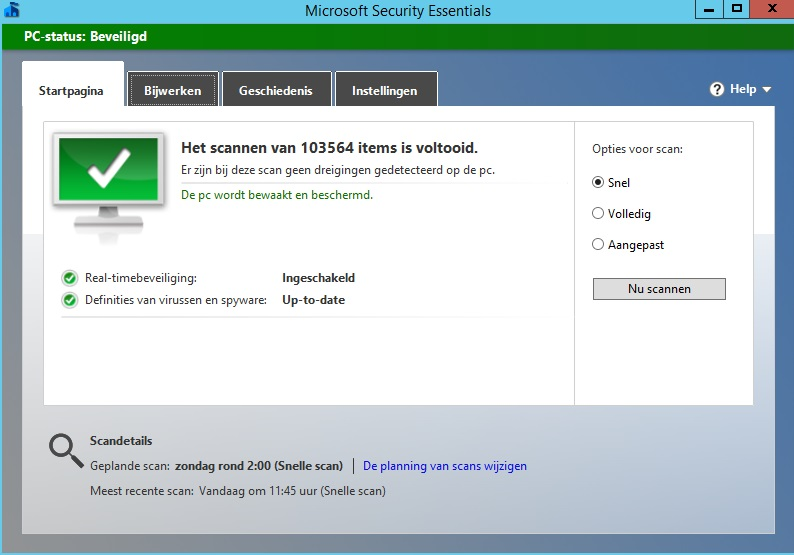
\includegraphics[scale=0.60]{img/AntiVirus}
\end{center}
\caption{Voorbeeld van succesvolle scan met volgende geplande scan}
\label{img:AntiVirus}
\end{figure}

\subsubsection{Regelmatig scannen en updaten}
Het spreekt voor zich dat deze anti-virus regelmatig moet ge-update worden zodat wanneer er een nieuwe bedreiging gesignaleerd wordt, deze direct kan toegevoegd worden aan de anti-virus software. Door het dagelijks uitvoeren van updates en een anti-virusscan blijft de server optimaal beschermt. Het beste is om dit 's nachts te doen als het netwerk niet gebruikt wordt om zo de gebruikers van het netwerk niet te belasten. 

\section{IIS best practices WebServer}
\subsection{Dedicated server}
Het is zeer belangrijk dat IIS een dedicated server is. Het is volgens \cite{Microsoft2013} gebruikelijk om de webserver apart van de domeincontroller te doen. Dit heeft als reden dat er geen lokale accounts zijn op een domeincontroller en deze lokale accounts zijn belangrijk voor een veilige IIS-server. Het samenplaatsen van een DC en een webserver beperkt de beveiligingsmogelijkeden enorm. Bijvoorbeeld een nieuwe exploit die door een hacker wordt gebruikt zal zo niet alleen de webserver aantasten, maar ook het hele netwerk. Daarom zijn deze twee dus het best gescheiden, zoals in deze opstelling het geval is.

\subsection{Inetpub}
De inetpub-map wordt bij elke installatie van IIS aangemaakt en standaard wordt die geplaatst op de C-schijf. Aangezien dit dezelfde schijf is waar het besturingssysteem opstaat, is het gebruikelijk om deze map op een aparte schijf te zetten zodat de toegang tot deze schijf beter kan beschermt worden. De schijf waar het besturingssysteem opstaat kan nooit zo goed beschermt worden als een aparte schijf. \citep{Darmanin2014}

\subsection{Modules}
In totaal bevat IIS meer dan 30 modules en deze moeten niet allemaal actief zijn. In de IIS manager kan er in het modulescherm van de geselecteerde website bepaalde modules op inactief gezet worden. In de lijst moet er beslist worden welke modules nodig zijn en de welke overbodig zijn. De overbodige modules kunnen dan worden uitgeschakeld door deze uit de lijst te verwijderen. In dit geval blijven alle modules staan want deze zijn nodig voor het uitvoeren van de applicatie. \citep{Darmanin2014} \citep{Microsoft2013}

\begin{figure}[H]
\begin{center}
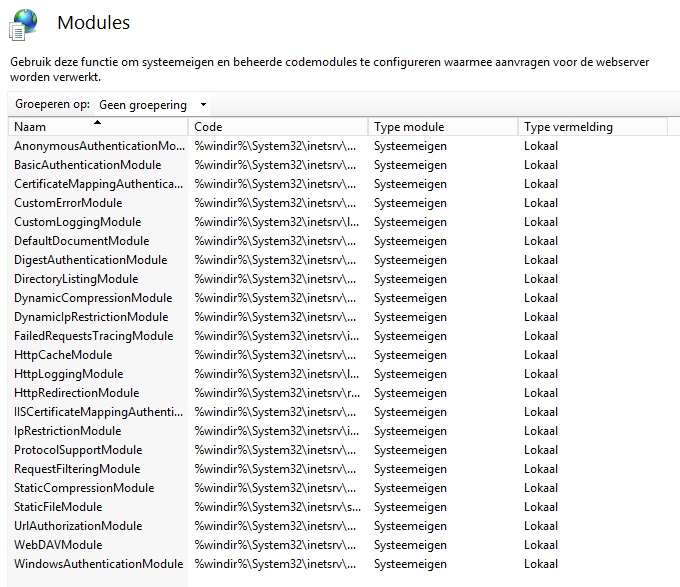
\includegraphics[scale=0.60]{img/IIS_Modules}
\end{center}
\caption{Alle modules die geactiveerd blijven}
\label{img:IISModules}
\end{figure}

\subsection{Opties methode uitschakelen}
De opties methode geeft een lijst van methodes weer die worden ondersteund door de webserver. Dit kan waardevolle informatie opleveren voor een hacker. Het is dan ook een best practice om deze methode uit te schakelen en dit gebeurd door het woord \textit{OPTIONS} uit te sluiten van de \textit{HTTP Verb request filtering rules} in IIS. Dit wordt gedaan door de website te selecteren in de IIS-manager en dan dubbel te klikken op \textit{aanvraagfiltering} en naar het tabblad \textit{HTTP-termen} te gaan. Hier wordt als actie gekozen \textit{Term weigeren...} en wordt \textit{OPTIONS} ingevuld en op OK gedrukt. Nu staat deze regel als enige in de lijst en is deze best practice in orde gebracht zoals in figuur~\ref{img:IISOptions} te zien is. \citep{Darmanin2014}

\begin{figure}[H]
\begin{center}
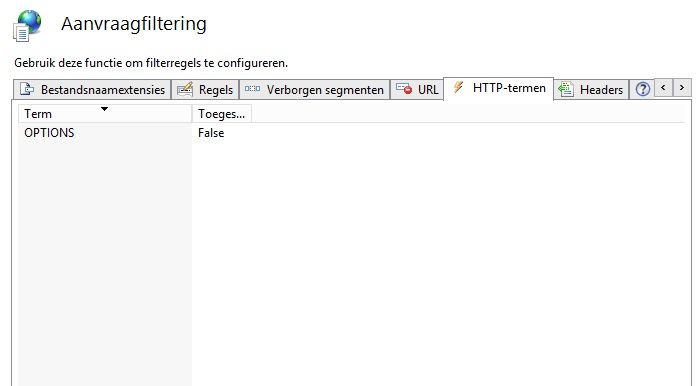
\includegraphics[scale=0.60]{img/IIS_Options}
\end{center}
\caption{De term OPTIONS wordt niet toegestaan}
\label{img:IISOptions}
\end{figure}

\subsection{Dynamische IP restricties}
Het inschakelen van dynamic IP restrictions module zorgt ervoor dat IP-adressen die een bepaald aantal requests hebben verzonden worden geblokkeerd. Hierdoor worden \textit{Denial of Service-aanvallen} voorkomen. Deze module inspecteert het IP-adres van elke request en zal deze requests filteren om de IP-adressen met slechte bedoelingen tijdelijk te blokkeren. Dit kan gedaan worden door naar de IIS-manager te gaan en de naam van de website te selecteren en te dubbelklikken op \textit{beperkingen voor IP-adressen en domeinen}. In het actie paneel wordt er geklikt op \textit{instellingen voor dynamische beperking bewerken.. }en kunnen er restricties ingevoerd worden. De eerste twee vakjes van de drie moeten worden aangevinkt en de waarden kunnen naar keuze ingevuld worden, in dit geval is 5-20-200 ingevuld. \citep{Darmanin2014}

\begin{figure}[H]
\begin{center}
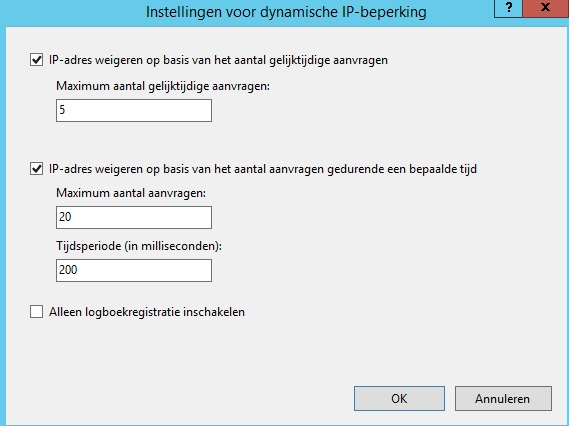
\includegraphics[scale=0.60]{img/IIS_Restrictie}
\end{center}
\label{img:IISRestrictie}
\caption{Instellingen voor dynamische IP-beperking}
\end{figure}

\subsection{Request Filtering Rules}
Het is altijd een goed idee om de verschillende types van HTTP-request die worden verwerkt door IIS te beperken. Door het instellen van uitsluitingen en regels kunnen potentieel gevaarlijke request er nooit doorkomen. Dit gebeurd in de IIS Manager waar de juiste website wordt gekozen en waarna er dubbel wordt geklikt op \textit{Requestfilters}. Hier wordt er gegaan naar het tabblad \textit{regels} en kunnen verschillende filterregels toegevoegd worden.\citep{Darmanin2014} \citep{Microsoft2013}

\subsection{Inschakkelen logs}
Door het in te schakelen van het IIS logsysteem worden verschillende HTTP-request gelogged. Indien er problemen voordoen dan kan er hier gekeken worden om een betere kennis te vergaren over het probleem. Dit kan vrij snel en simpel ingeschakeld worden door te gaan naar de IIS manager en daar de gewenste website te selecteren en op \textit{logging} te klikken. Best wordt er gekozen om een nieuw bestand aan te maken want deze bestanden groeien vrij snel. \citep{Darmanin2014} \citep{Microsoft2013}

\section{SQL Server best practices WebServer}
\subsection{Uitschakelen van onnodige features}
Nadat de software is geïnstalleerd wordt er best gegaan naar de \textit{SQL Server Configuration Manager Tool} om alle onnodige features te verwijderen. In dit geval zijn er geen extra features geïnstalleerd die niet gebruikt zijn dus hier is dit overbodig. \citep{Mam2013}

\subsection{Patchen en updaten}
Zoals elk Microsoft-product wordt ook SQL Server regelmatig voorzien van de nieuwste updates en patches om de applicatie zo goed mogelijk te beveiligen tegen hedendaagse aanvallen. Het is best dat deze updates eerst eens worden gedownload en geïnstalleerd in een testomgeving om daarna deze in de echte omgeving te implementeren. Dit kan voorkomen dat er bugs in de patch de server in gevaar brengen. \citep{Mam2013}

\subsection{Loggen van aanmeldpogingen}
Het kan zeer handig zijn om logbestanden bij te houden van iedereen die zich aanmeldt op de SQL Server. Zowel de gelukte als de mislukte login-pogingen zouden moeten geregistreerd worden. Dit kan gedaan worden door naar \textit{SQL Server Management Studio} te gaan en te rechterklikken op de gewenste SQL Server en dan de \textit{Eigenschappen} te selecteren. Aan de linkerkant is er dan de mogelijkheid om op \textit{Security} te klikken en daar kan er gekozen worden voor \textit{Both failed and successful logins}. Als dit is gedaan dan hoeft SQL enkel opnieuw worden opgestart en dan zal dit vanaf nu altijd gebeuren. \citep{Mam2013}

\chapter{Risico-analyse}
Het uitvoeren van een risico-analyse kan in verschillende stappen onderverdeeld worden. Allereerst moet er een opsomming zijn van alles \textit{assets} die zullen onderzocht worden in de risico-analyse. Dan kan er gebrainstormed worden om te kijken welke soort bedreigingen er voor de specifieke server zijn, in dit geval een webserver. Tot slot wordt er m.b.v. enkele tools en wat opzoekwerk gekeken naar welk van deze bedreigingen het belangrijkste zijn. Dit wil zeggen dat er wordt gekeken naar de kans dat deze voorvalt en de mogelijke schade die deze kan toebrengen en zo worden de bedreigingen dan gecatalogiseerd op het vlak van belang.

\section{Assets}
In dit geval wordt er gewerkt met een webserver waarop de recenste versie van Windows Server 2012 R2 staat geïnstalleerd met de volgende rollen/programma's/besturingssystemen op geïnstalleerd:
\begin{itemize}
	\item Windows Server 2012 R2 (waarde 10)
	\item Internet Information Services 8 (waarde 8)
	\item Externe toegang, routering (waarde 9)
	\item Microsoft SQL Server Express 2014 (waarde 7)
\end{itemize}
De waarde die aan deze assets wordt meegegeven, wordt verklaard in het volgende deel.

\section{Bedreigingen en risicofactor}
De soorten bedreigingen kunnen ingedeeld worden per laag van het TCP/IP-model. Hierdoor kan er structureel gekeken worden naar elke laag om zo te kijken welke bedreigingen er aanwezig zijn voordat er wordt verder gekeken. Deze werkwijze zorgt er ook voor dat er minder snel een bedreiging over het hoofd wordt gezien. Er wordt ook gekeken naar wat de mogelijkheid is dat deze aanvallen op een webserver zullen plaatsvinden en wat de mogelijke schade kan zijn en zo wordt er een cijfer meegegeven aan een aanval om te kijken hoe belangrijk deze is. Hoe hoger cijfer, hoe belangrijker het is om de server te beschermen tegen deze aanval. Het berekenen van dit cijfer gebeurd door deze formule: "`schade van de aanval x kans op een aanval"'. Beide factoren krijgen een cijfer van 1 tot 10 mee waar 10 de hoogste factor (meeste schade of grootste kans op een aanval) voorstelt en 1 dus het omgekeerde. \citep{Sim2005}

\subsection{Applicatielaag}
Dit is de 4de en de hoogste laag van het TCP/IP-model en is een samenvoeging van de applicatie -, presentatie -en sessielaag van het OSI-model. Deze laag bevat al de ''high-level'' protocollen zoals DNS, HTTP, Telnet, SSH, FTP, TFTP, SNMP, ... noem maar op. Deze laag heeft ook een rechtstreekse verbinding met de eindgebruiker en de applicaties. \citep{Thomas2013}

\subsubsection{Laag 7 DoS-aanvallen}
Een DoS-aanval (of Denial of Service-aanval) die zich afspeelt in de applicatielaag kan een hele server doen crashen. Dit kan gedaan worden door één gebruiker. Indien er meerdere personen samenwerken om een netwerk/server plat te leggen dan wordt er gesproken van een DDoS-aanval (of Distributed Denial of Service-aanval). Een voordeel van DDoS-aanvallen zijn dat deze moeilijker zijn om na te trekken aangezien er verschillende mensen op hetzelfde moment aanvallen i.p.v. één persoon bij een DoS-aanval. \citep{Blagov2014} Er zijn verschillende soorten applicatielaag DoS-aanvallen zoals RUDY (R-U-Dead-Yet) waar IIS 8 het slachtoffer wordt en XerXes waar de server via een TCP-connectie het slachtoffer wordt. \newline

De kans dat deze soort aanvallen zullen uitgevoerd worden is zeer groot aangezien het hier gaat over een webserver en die zijn een makkelijk doelwit voor zulke aanvallen. De factor \textit{kans op een aanval} krijgt dus een 9 mee. De schade die een DoS-aanval kan veroorzaken is niet mis, deze kan een server of webapplicatie helemaal offline halen zolang de aanval duurt. Het spreekt voor zich dat dit vrij irritant is, maar er is geen mogelijkheid tot diefstal van gegevens zoals kredietkaartgegevens of inloggegevens en er kan niets op de server of webapplicatie zelf worden veranderd dus de factor \textit{schade van de aanval} krijgt een 6 mee. Als dan de formule wordt uitgevoerd dan krijgt deze aanval de waarde \textbf{54} mee.

\subsubsection{DNS Poisoning}
Dit is een aanval die de cache van DNS ''vergiftigd'' door valse invoer te geven. Zo kan een aanvaller een willekeurige website als facebook of google laten verwijzen naar een IP-adres van zijn eigen website met malware om zo de gebruiker op te lichten. Als een hacker toegang verkrijgt tot een DNS-server en deze valse invoeren plaatst, kan elke persoon binnen een netwerk door het surfen naar een bepaalde website bij een verkeerde website terechtkomen of zelfs bij de machine van de aanvaller zonder dat deze persoon er zelf weet van heeft. Een hacker kan toegang verkrijgen tot een DNS-server door bijvoorbeeld foutjes uit te buiten die in de DNS-software zitten. \citep{Hoffm2015} \newline

Op een webserver is de kans dat dit soort aanvallen voorkomen immens klein omdat in de meeste gevallen een DNS-server en een Webserver gescheiden zullen zijn. Zoals eerder besproken is het een best practice om de domeincontroller en de webserver op aparte machines te plaatsen en DNS zit in het merendeel van de gevallen bij de domeincontroller. Hierdoor is krijgt de factor \textit{kans op een aanval} een 1 mee. De schade die deze aanval kan veroorzaken is echter zeer groot. Als een hacker het inlogportaal van een bank namaakt en de gebruiker hier via DNS poisining naartoe stuurt, kunnen zo bankgegevens gestolen worden en dit kan grote gevolgen hebben. Hierdoor krijgt deze aanval als factor \textit{schade van de aanval} een 9 mee. Dit brengt de totale waarde van de aanval naar de waarde \textbf{9}.

\subsubsection{SQL-injectie}
Een SQL-injectie is simpel uitgelegd een aanval die slechte code in een webapplicatie gebruikt om hackers SQL-commando's in te geven in een veld om zo toegang te verkrijgen tot een database. Zo kan een hacker bijvoorbeeld bepaalde SQL-commando's ingeven in het login formulier om zo persoonlijke gegevens van anderen te verkrijgen van in de database van de webapplicatie. Bij een succesvolle SQL-injectie kan een hacker niet alleen kijken naar gegevens in een database, hij kan deze gegevens zelfs verwijderen. Dit kan gebeuren bij elk invoerveld waar de gebruiker data moet invoeren om dan data terug te ontvangen. Als deze invoer niet gevalideerd wordt, dan is de kans reeël dat wanneer bijvoorbeeld het commando \begin{verbatim} SELECT * FROM USERS; DROP TABLE USERS;\end{verbatim} wordt ingegeven, dit ook effectief wordt uitgevoerd met alle gevolgen nadien. \citep{Acunetix2014} \newline

Volgens \cite{Acunetix2014} is een SQL-injectie één van de meest voorkomende aanvallen op de applicatielaag die vandaag voorkomen. Hierdoor is de kans dus vrij groot dat een webserver met een achterliggende webapplicatie hiermee te maken krijgt. Dus de factor \textit{kans op een aanval} krijgt hier ook een 10 mee. De schade die deze aanval kan veroorzaken is natuurlijk ook zeer groot. Een goed gecoördineerde SQL-injectie kan de inloggegevens van alle gebruikers stelen en kan zelfs velden van de database verwijderen. Hierdoor krijgt de factor \textit{schade van de aanval} een 9 mee. Dit brengt de totale waarde van de aanval op \textbf{90}, hetgeen zeer hoog is.

\subsubsection{Dictionary attack telnet}
In deze aanval wordt er gekeken via een port scan of poort 23 (telnet) open is bij een specifieke machine. Indien deze poort open is dat kan er via een \textit{dictionary attack} een juiste wachtwoord/gebruikersnaam-combinate gezocht worden om via poort 23 binnen te breken in een machine. Als dit gelukt is kan er via \textit{Putty} een verbinding worden gemaakt met de doelmachine. De tool die hier het best voor wordt gebruikt is \textit{Hydra}. Deze tool staat ook in elke Kali Linux-machine bij de top 10 meest gebruikte tools. \citep{Wilde2013} \newline

Dit is een aanval die niet moeilijk aan te leren is maar die wel veel tijd en oefening vergt en hierdoor neemt de kans op een aanval toch een beetje af. Toch krijgt deze aanval nog bij de factor \textit{kans op aanval} een 7 mee. De schade die deze aanval kan aanrichten is immens. Bij een succesvolle aanval zal de hacker volledige controle krijgen over het doelwit, in dit geval een webserver. Hij kon zo alle gegevens inkijken, kopiëren en verwijderen. Zo kan er gevoelige en geheime informatie doorgespeeld worden en kunnen er allerlei soorten chantage en spionage plaatsvinden. Bij de volledige controle over een machine zijn er veel zaken die een hacker kan doen dus hierdoor krijgt de factor \textit{schade van de aanval} een 10 mee. Hierdoor komt de totale waarde van deze aanval op een \textbf{70} te staan.

\subsection{Transportlaag}
Dit is de derde laag van het TCP/IP-model en is hetzelfde als de 4de laag van het OSI-model. Deze laag is vooral gekenmerkt door de twee transportprotocollen TCP en UDP die hier op werken. De bedoeling van deze laag is om foutvrije berichten te verzenden tussen hosts. \citep{Thomas2013}

\subsubsection{Port scanning}
Een port scan kan gebruikt worden als een aanval, maar kan ook gebruikt worden voor de administrator te helpen. Bij een port scan wordt er gekeken bij een computer of een netwerk welke TCP -en/of UDP-poorten er allemaal open zijn en luisteren. Als aanvaller kan er zo gekeken worden waardat er mogelijkheden zijn om in te breken en als administrator kan er gekeken worden naar de zwakke plekken in het netwerk of op een computer/server. Via een port scan kan een administrator ook zien of er \textit{bad ports} open zijn. Dit zijn poorten die open staan omdat er een trojan horse, DDoS-tool of een andere soort van kwaadaardige software op het systeem staat. Zo kan er ook tijdig ingegrepen worden. \citep{Kessler2001} \newline

Aangezien een webserver vanaf het openbare web bereikbaar is, is er een groot risico op port scans. Er bestaan zelfs bots die automatisch port scans uitvoeren bij willekeurige websites en alle zwaktes doorgeven aan de eigenaar. Hierdoor is de factor \textit{kans op aanval} een 9. De schade daarentegen is zeer laag want een port scan zelf brengt geen schade toe tot een netwerk en is zelfs niet illegaal. Het uitbuiten van de exploits die deze port scan blootlegt, dat is wel illegaal. Het enigste wat een port scan doet is kijken door het raam van het huis, hetgeen niet strafbaar is. Pas wanneer er wordt ingebroken dan pas is het strafbaar en kan er schade zijn. Hierdoor is de factor \textit{schade van de aanval} toch een 2 aangezien het potentiële zwaktes tentoonstelt. Dit brengt de totale waarde van deze aanval op \textbf{18}.

\subsubsection{TCP SYN flood} 
Deze aanval is een soort van DOS-aanval waar de aanvaller de bekende \textit{three-way handshake} misbruikt. Bij een normale three-way handshake wordt er een SYN-bericht gestuurd naar de server met de vraag om een connectie te verkrijgen. Daarna krijgt de gebruiker een SYN-ACK terug waarme zijn request wordt geaccepteerd. Tot slot antwoordt de gebruiker met een ACK waarme de verbinding tot stand wordt gebracht (zoals te zien is in figuur~\ref{img:ThreeWayHandshake}). Bij een TCP SYN flood-aanval worden er meerdere SYN-berichten verzonden en worden er meerdere SYN-ACK berichten terug gestuurd naar de gebruiker maar deze stuurt geen enkele keer een ACK-bericht terug. Hierdoor blijven er half open verbindingen openstaan op een server en wordt er geheugen gebruikt op de server. Een voorbeeld van deze aanval is \textit{Sockstress}. \citep{Rouse2014}    

\begin{figure}[H]
\begin{center}
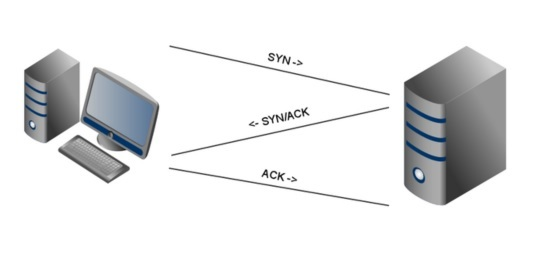
\includegraphics{img/ThreeWayHandshake}
\end{center}
\label{img:ThreeWayHandshake}
\captionsource{ThreeWayHandshake}{http://blogs.ixiacom.com/ixia-blog/tcp-portals-the-handshakes-a-lie/}
\end{figure}

Dit is een aanval die veel kan voorkomen en die ook door gerespecteerd lid van de security community \cite{Bown2013} als zeer gevaarlijk wordt beschouwd. Het feit dat de webserver rechtreeks in verbinding staat met het internet, wilt zeggen dat de kans zeer groot is dat deze aanval zal plaatsvinden dus daarom is de factor \textit{kans op aanval} een 9. Een succesvolle aanval kan een server doen vastlopen en ook al wordt de aanval gestopt, de server kan alleen maar terug werken nadat deze handmatig opnieuw is opgestart. Dit zorgt ervoor dat de webserver onbereikbaar is tot dat er iemand naar de locatie gaat en op de shutdown-knop drukt en de server weer laat rebooten. Deze aanval kan geen gevoelige gegevens wissen of stelen, maar kan wel voor een lange downtime zorgen van een website/server. Daarom krijgt deze aanval een 7 mee bij de factor \textit{schade van de aanval}. Hierdoor komt de waarde van deze aanval op \textbf{63} te staan.

\subsection{Internetlaag}
De internetlaag is de tweede laag van het TCP/IP-model en staat gelijk aan de 3de laag, de netwerklaag, in het OSI-model. Deze laag steekt de data in pakketten genaamd IP-datagrammen waar de bron -en eindbestemming van het pakket in verwerkt zitten. Deze laag is ook verantwoordelijk voor het routeren van deze pakketten. De protocollen die vooral worden gebruikt op deze laag zijn IP, ICMP en ARP. \citep{Thomas2013}

\subsubsection{Ping flood}
Een Ping flood is eigenlijk de oudste en meest primitieve vorm van een DOS-aanval want iedereen kan het doen en het is extreem gemakkelijk. Als een server een Ping flood-aanval te verduren krijgt, dan krijgt deze server zoveel ping requests dat deze het niet meer aankan omdat er teveel CPU-resources gebruikt worden. De aanvaller stuurt dan pings, via ICMP-pakketten, zonder te wachten op een antwoord. Hierdoor kan de server niet tijdig antwoorden en worden echte requests ook geblokkeerd. Dit kan leiden tot een immens vertraagde server en/of website. \citep{Grid2010}

Bij een webserver hebben deze soort aanvallen een grote kans om uitgevoerd te worden door de verbinding die deze server heeft met het internet en omdat het zo gemakkelijk is om uit te voeren. Om een soortgelijke aanval te doen heeft een persoon weinig kennis nodig, dit maakt deze aanval zo angstaanjagend omdat iedereen het zou kunnen na een tutorial van 5 minuten. Hierdoor krijgt de factor \textit{kans op aanval} een 10. De schade die deze aanval kan veroorzaken is echter vrij bescheiden. Het is niet dat een soortgelijke aanval een server kan plat gooien, maar het kan wel voor de nodige vertraging zorgen. Dit kan ervoor zorgen dat de website of server veel trager zal reageren op requests en dat de netwerkverbinding veel trager zal gaan. Aangezien deze aanval geen permanente schade kan veroorzaken maar enkel overlast, krijgt deze bij de factor \textit{schade van de aanval} een 3 mee. Hiermee komt de totale waarde van de aanval op \textbf{30}.

\subsubsection{ARP spoofing - Man in the middle}
Deze aanval wordt ook wel eens \textit{ARP cache poisoning} of \textit{ARP poison routing} genoemd. Dit is een aanval waar een aanval valse Address Resolution Protocol-berichten (ARP) over een LAN verzendt. Dit heeft als resultaat dat het MAC-adres van de aanvaller wordt gelinkt met een IP-adres van een echte computer in het netwerk. Vanaf deze link is geslaagd, zal de aanvaller alle data ontvangen die is bedoeld voor de computer waarvan de aanvaller het IP-adres gebruikt. De Man in the middle-aanval is de variant van ARP spoofing waar het verkeer tussen twee hosts eerst naar de hacker zijn machine wordt verzonden en nadat deze persoon de pakketten heeft kunnen bekijken (sniffen), dan wordt het verkeer naar de normale bestemming verzonden. Dit gebeurd zonder dat iemand er weet van heeft. Deze aanval kan alleen gebruikt worden, maar wordt in vele gevallen ook gebruikt in combinatie met een andere aanval. Bij een DoS-aanval kan ARP spoofing worden gebruikt om meerdere IP-adressen te linken aan één MAC-adres en zo het verkeer van al deze IP-adressen naar het doelsysteem waar het MAC-adres van is gebruikt. Zo wordt het doel overspoeld met verkeer. \citep{Glynn2014} \newline

Een soortgelijke aanval kan voorkomen op een webserver omdat deze rechtstreeks in verbinding staat met de router, maar deze is echter niet zo makkelijk uit te voeren als een ping flood. Hierdoor krijgt deze aanval bij de factor \textit{kans op aanval} een 8. De schade die een hacker kan toebrengen aan een server of netwerk is dan weer vrij groot. Zo kan deze alle pakketten die worden verstuurd naar een ''vergiftigde'' host om zo gevoelige informatie te verkrijgen. Als een hacker de verbinding tussen bijvoorbeeld de baas en onderbaas van bedrijf A aanvalt, dan kan deze al het verkeer dat deze twee tussen elkaar uitwisselen inkijken zonder dat er iemand weet van heeft. Als deze personen dan gevoelige informatie uitwisselen met elkaar kan dit grote gevolgen hebben. Dit is dus een vrij gevaarlijke aanval die niet direct kan worden opgemerkt dus deze krijgt als factor \textit{schade van de aanval} een 9. Dit brengt de totale waarde van deze aanval op \textbf{72}.

\subsection{Netwerktoeganglaag}
Dit is laag 1 van het TCP/IP-model en is een samenvoeging van de fysieke -en datalinklaag bij het OSI-model, die daar laag 1 en 2 zijn. Hier worden de details meegegeven over hoe data precies over een netwerk moet verzonden worden. De protocollen die hier het meeste voorkomen zijn Ethernet, Token Ring en Frame Relay. 

\subsubsection{Keylogging}
Bij dit soort aanvallen wordt input van het toetsenbord opgeslagen zonder dat de gebruiker dit doorheeft. Deze aanval wordt vooral gebruikt om zo aan wachtwoorden en gevoelige informatie te komen. Keylogging hoeft ook niet direct illegaal te zijn, er zijn veel varianten van keylogging die in softwareprogramma's worden gebruikt om zo een beter egebruikerservaring aan te bieden. Ook is er legale software waarmee administrators kunnen meekijken met wat de gebruikers op een netwerk allemaal doen. Natuurlijk is de lijn tussen het controleren van de werknemers en spionage een dunne lijn. Legale software kan zo ook gebruikt worden om illegale zaken uit te voeren. In tegenstelling tot de meeste aanvallen die eerder al besproken zijn, kan software voor deze aanval op de vrije markt gekocht worden en dat maakt het ook gevaarlijker. Bij een soortgelijke aanval krijgt een hacker de keylogger-software op de doelmachine en kan zo wachtwoorden of bankinformatie te weten komen. Een bekend voorbeeld van deze aanval is het keylogger-incident bij een grote Scandinavische bank waar 1 miljoen dollar is gestolen van bepaalde accounts. De aanvaller stuurde mails in de naam van de bank naar bepaalde klanten met de melding dat deze nieuwe anti-spamsoftware moesten installeren. Bij het downloaden van de bijlage werd er een keylogger geïnstalleerd en zo kreeg de aanvaller de bankinformatie van al deze klanten. \citep{Grebennikov2007} \newline
 
Deze soort aanval is niet moeilijk om uit te voeren en komt vrij veel voor. Op een server zal deze echter veel minder voorkomen aangezien er op een server zo goed als nooit bestanden zullen gedownload worden van het internet of e-mails en al zeker niet van niet-vertrouwde bronnen. Een keylogging-aanval zal vooral plaatsvinden op een client. Hierdoor krijgt de factor \textit{kans op aanval} een 2 mee. De schade die deze aanval kan aanrichten is dan weer vrij groot. Als een server/computer slachtoffer wordt van een keylogging aanval, kunnen wachtwoorden en gebruikersnamen gestolen worden om zo veel schade aan te richten of gevoelige informatie te stelen. Hierdoor krijgt de factor \textit{schade van de aanval} een 9 mee. De totale waarde van deze aanval komt dan op \textbf{18} te staan.

\section{Prioriteiten}
Nu er een opsomming is gemaakt van de verschillende bedreigingen kunnen er prioriteiten gesteld worden bij het onderzoeken van al deze bedreigingen. Er kan nu een tabel gemaakt worden met de naam van de bedreiging en de bijhorende waarde die deze heeft megekregen. Hoe groter de waarde, hoe hoger de aanval in de tabel zal geplaatst worden. Zo kunnen de aanvallen met het grootste risicogehalte eerst onderzocht worden.

\begin{table}[h]
\centering
\begin{tabular}{|l|l|}
\hline
\textbf{Bedreiging}              & \textbf{Risicowaarde} \\ \hline
SQL-injectie                     & 90                    \\ \hline
ARP spoofing - Man in the middle & 72                    \\ \hline
Dictionary attack telnet         & 70                    \\ \hline
TCP SYN flood                    & 63                    \\ \hline
Laag 7 DoS-aanvallen             & 54                    \\ \hline
Ping flood                       & 30                    \\ \hline
Port Scanning                    & 18                    \\ \hline
Keylogging                       & 18                    \\ \hline
DNS Poisoning                    & 9                     \\ \hline
\end{tabular}
\caption{Ordening bedreiging op risicogehalte}
\label{RisicoTabel}
\end{table}


\chapter{Penetration Testing}
%Hier ga ik verschillende aanvallen doen op deze server, zowel intern als extern, en ga ik mijn bevindingen noteren. Als de aanval slaagt, dan ga ik er een oplossing voor zoeken en 
%de oplossing testen, als de aanval niet slaagt, dan zijn de best practises voldoende.

\section{SQL-injectie}



\section{ARP Spoofing - Man in the middle}


\subsection{Uitvoering}
Om deze aanval uit te voeren staan er best drie terminalvenster open



\section{Dictionary attack telnet}
Telnet wordt in het algemeen gezien als onveilig en wordt daarom niet zoveel meer gebruikt. De variant van telnet, genaamd ssh, wordt veel meer gebruikt. Dit voorbeeld kan ook toegepast worden op dezelfde manier bij ssh, het enige verschil is dat het poortnummer van ssh nummer 22 is i.p.v. 23 voor telnet. Bij een portscan kunnen nog andere poorten gebruikt worden om binnen te breken via Hydra, maar in dit geval wordt er gefocussed op telnet

\subsection{Uitvoering}
Voor deze aanval uit te voeren moeten er in de Kali Aanvaller-machine twee terminalvensters geopend worden. In het eerste venster wordt er gestart met een port scan van het slachtoffer, in dit geval de webserver. Dit wordt gedaan door volgende lijn code in te geven:
\begin{verbatim} nmap 192.168.1.3 \end{verbatim}
Dit is het IP-adres van de webserver en dit zou een lijst moeten weergeven zoals in figuur~\ref{img:PortScan} is te zien. Er is echter maar één waarde belangrijk in deze lijst en dat is poort 23/tcp waar de service TELNET op draait. Dit wil zeggen dat de poort open staat.

\begin{figure}[H]
\begin{center}
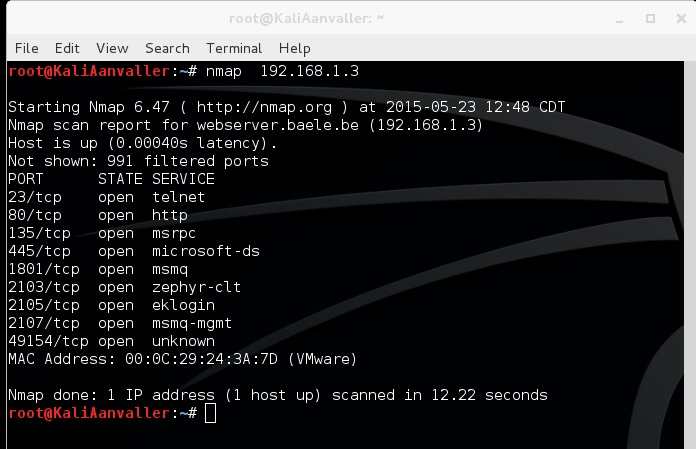
\includegraphics[scale=0.60]{img/HydraPortscan}
\end{center}
\caption{Resultaat van een port scan van de webserver}
\label{img:PortScan}
\end{figure}

In het andere terminalvenster kan nu de hydra-aanval uitgevoerd worden. Dit gebeurt met de volgende lijn:
\begin{verbatim} hydra -t 1 -l Administrator -P /root/test.txt -vV 192.168.1.3 telnet \end{verbatim}
In deze lijn code wordt er de inlognaam van het Administrator-account meegegeven. Standaard is dit \textit{Administrator} maar in de meeste gevallen zal dit een andere naam zijn. Daarna wordt er een bestand meegegeven genaamd test.txt waar er een hele lijst met wachtwoorden in zit. Deze lijst wordt dan volledig overlopen tijdens de aanval. Ten slotte wordt nog het IP-adres van het slachtoffer meegegeven en de service waarmee de aanval zich moet verbinden wat in dit geval \textit{telnet} is. Na het uitvoeren van deze aanval zullen alle mogelijke combinaties geprobeerd worden zoals te zien is in figuur~\ref{img:HydraAanval} en als er een positieve match is tussen gebruikersnaam en wachtwoord dan worden deze in het groen aangetoond zoals in figuur~\ref{img:HydraGeslaagd} te zien is. \citep{Moon2013}

\begin{figure}[H]
\begin{center}
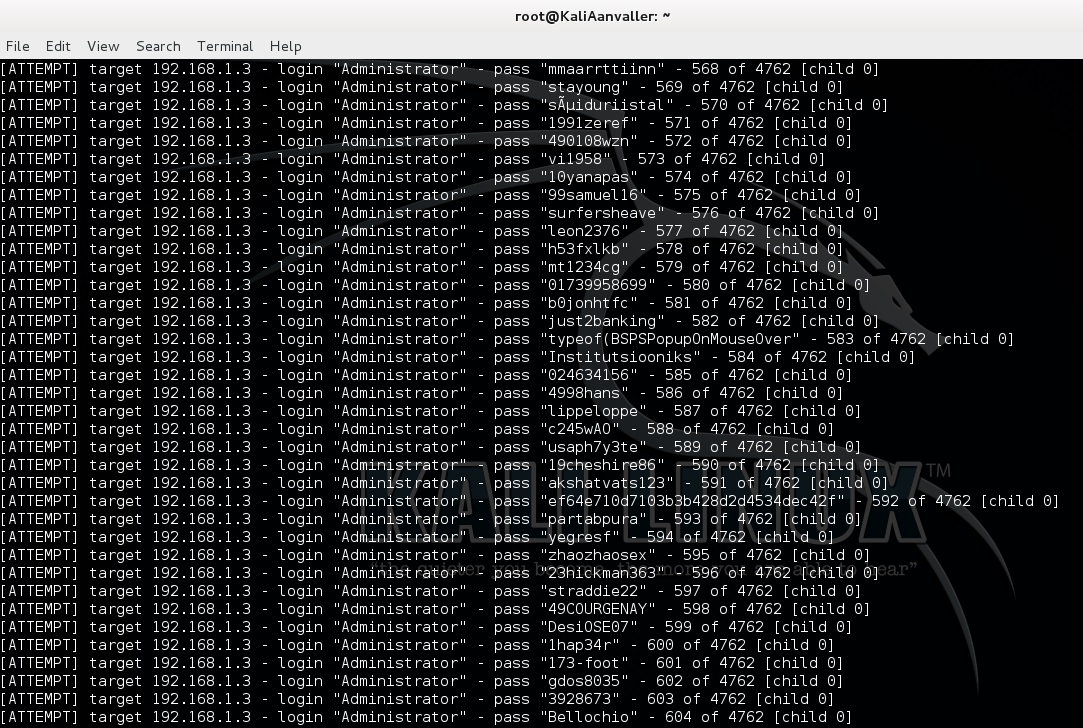
\includegraphics[scale=0.40]{img/HydraAanval}
\end{center}
\caption{Woordenlijst wordt doorlopen.}
\label{img:HydraAanval}
\end{figure}

\begin{figure}[H]
\begin{center}
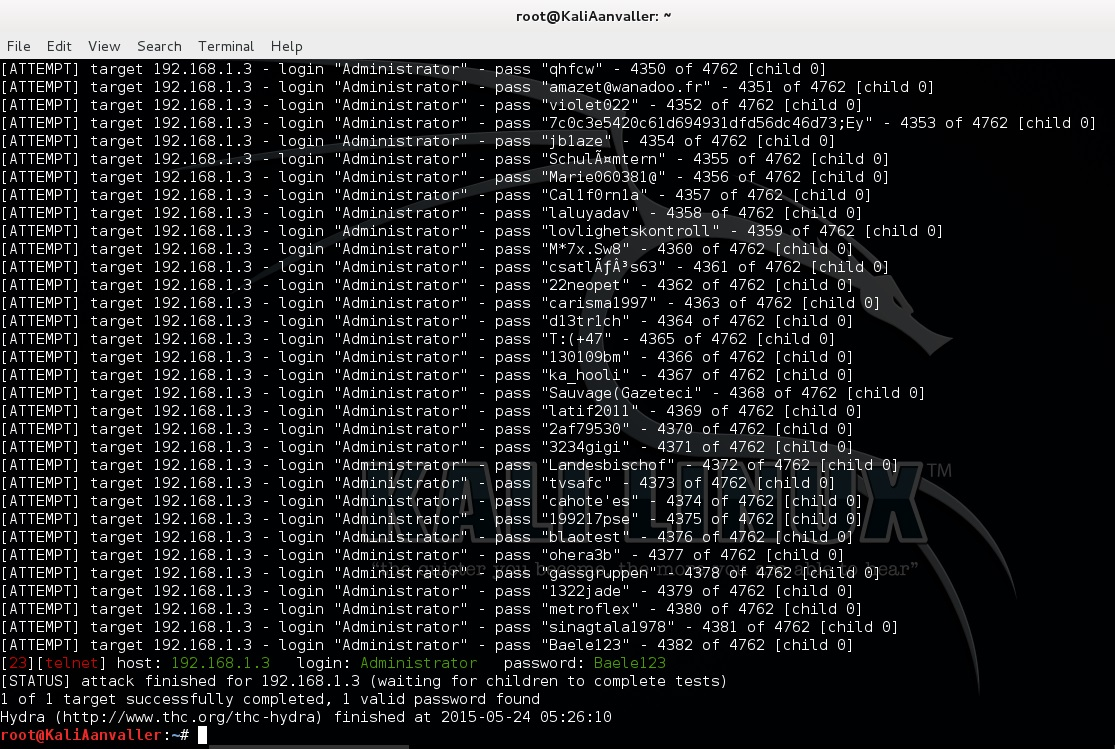
\includegraphics[scale=0.40]{img/HydraGeslaagd}
\end{center}
\caption{Er is een match gevonden.}
\label{img:HydraGeslaagd}
\end{figure}

Hierna kan er met de net verkregen inloggegeven ingelogged worden via het programma \textit{Putty}. Hier wordt er het slachtoffer IP-adres ingevoerd en wordt er gekozen voor poort 23 om daarna de inloggegevens in te vullen. Als deze kloppen dan komt er een verbinding tot stand met het slachtoffer zoals in figuur~\ref{img:HydraPutty} te zien is. Nu heeft de aanvaller volledige controle over de machine.

\begin{figure}[H]
\begin{center}
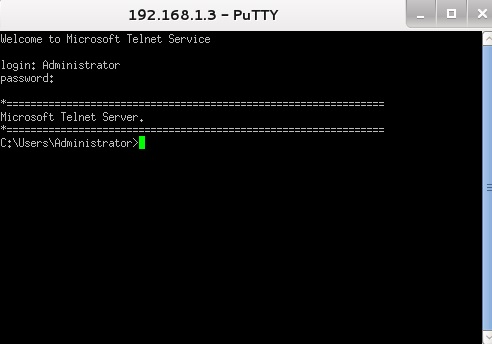
\includegraphics[scale=0.80]{img/HydraPutty}
\end{center}
\caption{Toegang tot de server via putty.}
\label{img:Putty}
\end{figure}

\subsection{Resultaten en beveiliging}
Deze aanval is geslaagd, maar dit is zonder rekening te houden met de best practices. Indien de best practices met betrekking tot het wachtwoord -en accountbeleid van kracht zijn dan heeft deze aanval veel minder kans op slagen. Bij het kiezen van een complex wachtwoord met voldoende tekens zal er veel meer tijd inkruipen om een woordenlijst te doorlopen. Hij het uitschakelen van het administratoraccount en het aanmaken van een nieuw account is er ook al specifieke voorkennis vereist om deze aanval aan te doen of de aanvaller zal moeten gokken. Een woordenlijst met potentiële namen voor een administratoraccount kan eventueel ook toegevoegd worden in dit geval, maar dit neemt ook extra tijd in beslag voor de hacker. Natuurlijk kan er nog een extra best practice worden toegevoegd en dat is om niet onnodige applicatie op de server te installeren. Als telnet of ssh of een ander alternatief nodig zijn, dan zijn de vooropgestelde best practices aan te raden. Indien deze software niet nodig is dan moet deze niet onnodig geïnstalleerd worden, dit geeft een hacker alleen maar mogelijkheden om binnen te breken.


\section{TCP SYN flood}
In deze aanval gaat Sockstress gebruikt worden, dit is één tool die kan gebruikt worden om een TCP SYN flood aanval uit te voeren. Allereerst moet er terug een port scan uitgevoerd worden om te kijken welke poorten er open zijn. Dit zal dezelfde uitvoer hebben als figuur~\ref{img:PortScan}. Alle poorten die hier zichtbaar zijn worden best even ergens genoteerd omdat deze later nog gebruikt zullen worden. Om deze aanval uit te voeren via de Kali Aanvaller-machine moet sockstress eerst gedownload worden aangezien dit niet standaard op Kali Linux staat. Dit wordt gedaan door de volgende lijnen code:
\begin{verbatim} apt-get update \end{verbatim}
\begin{verbatim} apt-get install libpcap0.8 libssl-dev -y \end{verbatim}
\begin{verbatim} wget http://samsclass.info/123/proj10/sockstress-outpost24.tar.gz \end{verbatim}
Indien dit commando niet werkt kan er gegaan worden naar \url{https://defuse.ca/sockstress.htm} waar sockstress ook kan gedownload worden.
\begin{verbatim} tar xzf sockstress-outpost24.tar.gz \end{verbatim}
\begin{verbatim} cd sockstress \end{verbatim}
\begin{verbatim} ./configure \end{verbatim}
\begin{verbatim} nano config.h \end{verbatim}
Met dat laatste lijntje wordt er in het configuratiebestand gegaan en daar moet \textit{\#include <pcap.h>} aangepast worden naar \textit{\#include </usr/include/pcap.h>}. Nu dit is aangepast kan de effectieve aanval worden uitgevoerd. Dit wordt gedaan met volgende lijn code:
\begin{verbatim} ./sockstress -A -c -1 -d 192.168.1.3 -m -1 -Ms -p 23,80,135,445,
1801,2103,2105,2107,49154,49176 -r 100000 -s 192.168.2.0/24 -vv
 \end{verbatim}
Nu kan er naar de webserver gegaan worden om in het taakbeheer te kijken naar de prestaties van het geheugen om te kijken of de aanval is geslaagd. In figuur~\ref{img:SockVoor} is het geheugen te zien voor de aanval en in figuur~\ref{img:SockNa} het geheugen na de aanval. Het geheugen is helemaal volgelopen en er kan niets meer gebeuren op de server, deze moet nu handmatig worden afgesloten.

\begin{figure}[H]
\begin{center}
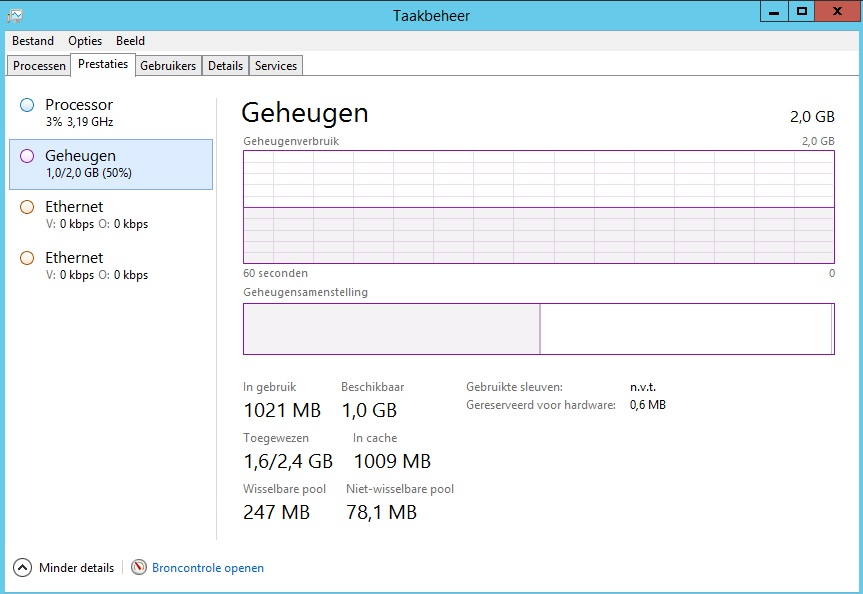
\includegraphics[scale=0.50]{img/SockVoor}
\end{center}
\caption{Gebruikt geheugen voor sockstress-aanval.}
\label{img:SockVoor}
\end{figure}

\begin{figure}[H]
\begin{center}
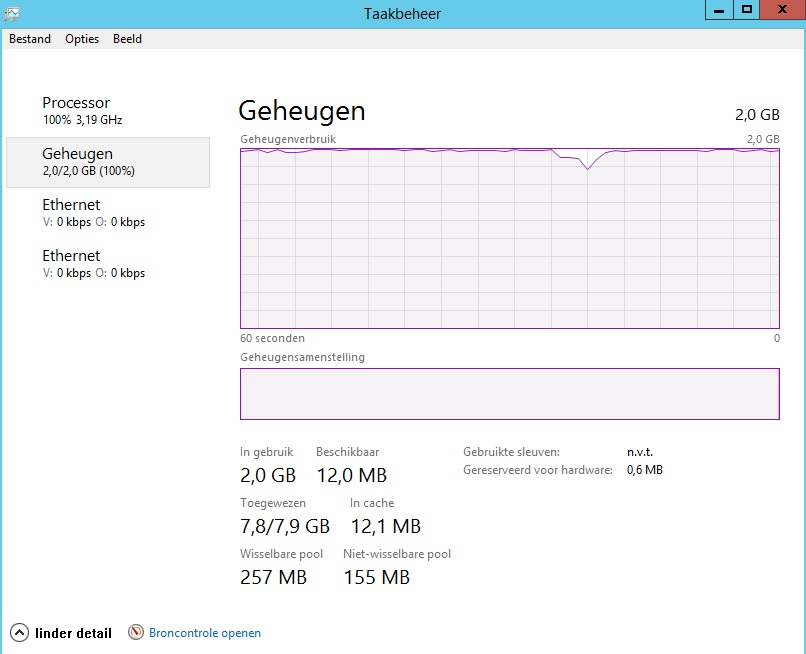
\includegraphics[scale=0.50]{img/SockNa}
\end{center}
\caption{Gebruikt geheugen na sockstress-aanval.}
\label{img:SockNa}
\end{figure}

\subsection{Resultaten en beveiliging}
Het gevolg van deze aanval is dat het RAM-geheugen helemaal is volgelopen zoals te zien is in figuur~\ref{img:SockNa} en dat er op de server niets meer kan gedaan worden. Deze kan ook niet via een remote verbinding worden afgesloten, dit moet effectief handmatig gebeuren. Indien de server een virtuele machine is dan moet er op \textit{Power Off} geklikt worden. Dit kan ervoor zorgen dat alle niet opgeslagen zaken verloren gaan....... 












\chapter{Post mortem}
%Hier ga ik een aanval uitvoeren en ga ik kijken waar je dit precies kan terugvinden als administrator of waar je kan het kan zien als het aan het gebeuren is.
\section{Manueel}
\subsection{RAM-geheugen}
Manueel kan er makkelijk gekeken worden naar het RAM-geheugen dat wordt gebruikt door "`ctrl+alt+del"' in te drukken of door met de rechtermuisknop te drukken op het Windows-logo linksonder op het scherm en "`Taakbeheer"' te selecteren. Hierin zijn er verschillende tabbladen en het RAM-geheugen kan gevonden worden in het tabblad "`Prestaties"' waarna er kan geklikt worden op "`Geheugen"' in de linkerkolom. In dit venster is het geheugengebruik voor de laatste 60 seconden zichtbaar en wordt deze elke seconden ververst. Als de curve per seconde omhoog gaat dan kan er sprake zijn van een Sockstress DDOS-aanval en kan er tijdig gehandeld worden. Het manueel bekijken van het RAM-geheugen kan handig zijn als de server opeens trager begint te werken om te kijken of het probleem niet hier ligt.

\subsection{Geblokkeerde accounts}
Na 3 foutieve inlogpogingen wordt een gebruikersaccount direct in een "`lock"' gestoken en moet deze door de administrator, of iemand met de benodigde rechten, weer uit deze lock gehaald worden. Om te kijken hoeveel en welke accounts er precies in een lock zitten, kan een zeer simpel powershell-commando uitgevoerd worden. Bij het openen van Powershell en met het volgende lijntje code worden alle geblokkeerde accounts weergegeven: "`Search-ADAccount -LockedOut"'. \newline 

Als alle accounts die in een lock zitten we op actief mogen staan, kan dit ook gedaan worden met een simpel lijntje code: "`Search-ADAccount -LockedOut | Unlock-ADAccount"'. Indien niet alle accounts terug actief mogen worden, kan er nog een stukje toegevoegd worden aan de code zodat er voor elk gelocked account een bevestiging moet gegeven worden: "`Search-ADAccount -LockedOut | Unlock-ADAccount -Confirm"'. Voor de accounts die weer op actief mogen staan moet er een "`y"' ingestyped worden en voor de accounts die in een lock moeten blijven wordt er een "`n"' getyped.

\subsection{Malware}
Om manueel te kijken of er malware aanwezig is op de server is er anti-virus-software nodig. Er zijn honderden verschillende keuzes en bij elke keuze kan er manueel een scan gestart worden en kan er manueel gekeken worden welke bedreigingen er gevonden zijn en welke risico's er aanwezig zijn. Deze kunnen dan manueel verwijderd of in quarantaine geplaatst worden. 

\section{Automatisch}
\subsection{Prestatiemeter}
Met behulp van de prestatiemeter-tool kunnen bepaalde zaken makkelijk in de gaten gehouden worden. In de prestatiemeter kunnen er gegevensverzamelaarset aangemaakt worden naar persoonlijke voorkeur die het mogelijk maken om elk aspect apart onder de loep te nemen en deze in log files op de slaan.

\subsubsection{RAM-geheugen}
De eerste gegevensverzamelaarset die zeer handig is om te maken is één die het gebruik van het RAM-geheugen in de gaten houdt. Deze kan worden ingesteld door allereerst naar de tool "`prestatiemeter"' te gaan en te rechterklikken op "`Prestatiemeter"' onder het tabblad "`controlehulpprogramma's"'. Daarna moet er onder de keuze "`Nieuw"' gekozen worden voor "`gegevensverzamelaarset"'. Nu kan er een gepaste naam gekozen worden voor deze set, in dit geval is "`RAMGeheugen"' een goede naam aangezien we hier het RAM-geheugen gaan bekijken. Bij de volgende keuzes mag er 2x op "`volgende"' gedrukt worden. \newline

Nu is de set aangemaakt en is deze terug te vinden onder het tabblad "`Gedefinieerd door de gebruiker"' en moet er hier op gedubelklikt worden tot "`Logboek voor Systeemmonitor"' zichtbaar is en dan moet er hier op gedubbelklikt worden. Nu zijn de eigenschappen van de set zichtbaar en kunnen er via "`Toevoegen"' specifieke paramters toegevoegd worden. In dit geval is het handig om naar "`Geheugen"' te gaan en daar te kiezen voor "`Beschikbare megabytes"' en "`Percentage toegewezen bytes in gebruik"'.	Nadat deze zaken zijn toegevoegd kan er 2x geklikt worden op de OK-knop. Nu moet er met de rechtermuisknop op de juist aangemaakt set geklikt worden om dan op "`starten"' te klikken, dit een 10-tal minuten te laten lopen en daarna op "`stoppen"' te drukken. Nu kan er gekeken worden naar het tabblad "`rapporten"' en "`gedefinieerd door de gebruiker"' naar wat deze actie juist heeft opgebracht. In dit scherm is er een bestand zichtbaar (met de bijhorende datum) die bij het dubbeklikken alle paramters laat zien met de bijhorende tijd in een mooie grafiek. Hier is duidelijk wanneer precies er pieken zijn in het gebruik van het RAM-geheugen en wanneer deze precies een bepaalde grens overschrijdt.

\subsubsection{foutieve inlogpogingen}
Het is mogelijk om foutieve aanmeldpogingen op de server te registreren in logbestanden. Dit kan gedaan worden door naar het "`lokaal beveiligingsbeleid"' te gaan en daar in de beveiligingsinstellingen bij "`lokaal beleid"' en "`controlebeleid"' kan er gekozen worden voor "`aanmeldingsgebeurtenissen controleren"'. Hierin kan er gekozen worden om mislukte pogingen te registreren. Hetzelfde wordt gedaan voor "`accountbeheer controleren"'. Elke keer dat er nu iemand wilt inloggen en deze geeft een foutief antwoord, dan wordt er een logbestand aangemaakt. 

\chapter{Conclusie}
\label{ch:conclusie}

% TODO: Trek een duidelijke conclusie, in de vorm van een antwoord op de
% onderzoeksvra(a)g(en). Reflecteer kritisch over het resultaat. Zijn er
% zaken die nog niet duidelijk zijn? Heeft het ondezoek geleid tot nieuwe
% vragen die uitnodigen tot verder onderzoek?
De conclusie zal geschreven worden na de feedback, als de laatste wijzingen uitgevoerd zijn!


\bibliographystyle{apa}
\bibliography{NathanBP}

%%---------- Back matter -------------------------------------------------

\listoffigures
\listoftables

\end{document}
